\documentclass[runningheads]{llncs}

\usepackage[T1]{fontenc}
\usepackage{graphicx}
\usepackage{amsmath, amssymb}
\usepackage{subcaption}
\usepackage{booktabs}
\usepackage{hyperref}
\usepackage{xcolor}

\graphicspath{{figures/}}

\begin{document}

\title{Disentangling Model and Human Data Uncertainty in Apparent Facial Age Estimation}

\titlerunning{Disentangling Uncertainty in Apparent Facial Age Estimation}

\author{Andrei Foitos\inst{1} \and
Ivo de Jong\inst{1} \and
Matias Valdenegro-Toro\inst{1}}

\authorrunning{A. Foitos et al.}

\institute{Bernoulli Institute for Mathematics, Computer Science and Artificial Intelligence,\\
University of Groningen, The Netherlands\\
\email{a.foitos@student.rug.nl, \{i.p.de.jong, m.a.valdenegro.toro\}@rug.nl}}

\maketitle

\begin{abstract}
Estimating the apparent age of individuals from facial images is challenging due to the subjective nature of perception and the inherent variability of the data. We investigate the role of uncertainty estimation, attributing uncertainty jointly to a lack of knowledge (epistemic) or inherent noise/chance (aleatoric). Leveraging the APPA-REAL dataset, we train Bayesian Neural Networks on datasets of varying sizes using three BNN approximations: MC-DropConnect, Flipout, and Deep Ensembles using supervision on human aleatoric uncertainty available in the APPA-REAL dataset. Each model outputs both the predicted apparent age and the amount of aleatoric and epistemic uncertainty. Our results confirm the hypothesis that the inherent aleatoric uncertainty remains stable across dataset sizes, while epistemic uncertainty increases as training data decreases. We further evaluate the trained models on UTKFace, a chronological-age dataset captured in the wild, and analyse generalisation through calibration and qualitative examples. These findings demonstrate that different sources of uncertainty can be quantified in face age estimation and that the learned uncertainties remain informative under distribution shift.

\keywords{Apparent age estimation \and Uncertainty quantification \and Bayesian neural networks \and Calibration \and Generalisation.}
\end{abstract}

\section{Introduction}
\label{sec:intro}

Artificial intelligence and machine learning systems are becoming increasingly integral to real-world decision-making~\cite{mckinsey2024}. While the predictive capabilities of modern models are impressive, their adoption in sensitive applications often hinges on more than just accuracy. It is also required to understand the reliability of those predictions. In high-stakes contexts, a wrong or overly confident prediction can have serious consequences. Thus, there is a growing demand for machine learning models that not only make predictions but also quantify their uncertainty~\cite{lakshminarayanan2017simple,gawlikowski2021survey,ribeiro2016should}.

One application area where prediction uncertainty is particularly relevant is facial age estimation, the task of predicting a person's age based solely on a facial image~\cite{fu2010age}. These models estimate the apparent age of a person, based on visual features of aging, rather than their actual chronological age~\cite{escalera2015chalearn}. Apparent age estimation introduces a layer of complexity: apparent age is subjective and often has a large degree of uncertainty. Human annotators may disagree due to individual bias or cultural perception~\cite{agustsson2017wild,escalera2017chalearn}, or consider multiple answers to be valid.

Machine learning regression models typically only output a single most likely value. In scenarios where there is no single correct answer~-- including apparent age estimation~-- this is insufficient. Instead, a model should give a most-likely estimate, and estimate the variance of which ages are likely. This is important for applications where age estimation is used to support the enforcement of age-restricted content or purchases.

With Uncertainty Quantification (UQ), the model not only outputs the most likely age but also provides an estimate of uncertainty~\cite{he2023survey}. There are two causes why a Machine Learning model (or anything) can be uncertain. These are aleatoric uncertainty and epistemic uncertainty~\cite{hullermeier2021aleatoric}. Aleatoric uncertainty is `chance' uncertainty. It is not always possible to estimate the exact apparent age of a person based on their face. This causes uncertainty, because the correct answer is not knowable. Epistemic uncertainty is `knowledge' uncertainty. This is uncertainty because the model has not sufficiently learned to estimate age reliably. If the model is trained more on data like this, it will get better estimates. Aleatoric uncertainty is therefore also considered as irreducible uncertainty, while epistemic uncertainty is reducible.

\begin{figure}[t]
\centering
\begin{subfigure}[t]{0.48\linewidth}
\centering
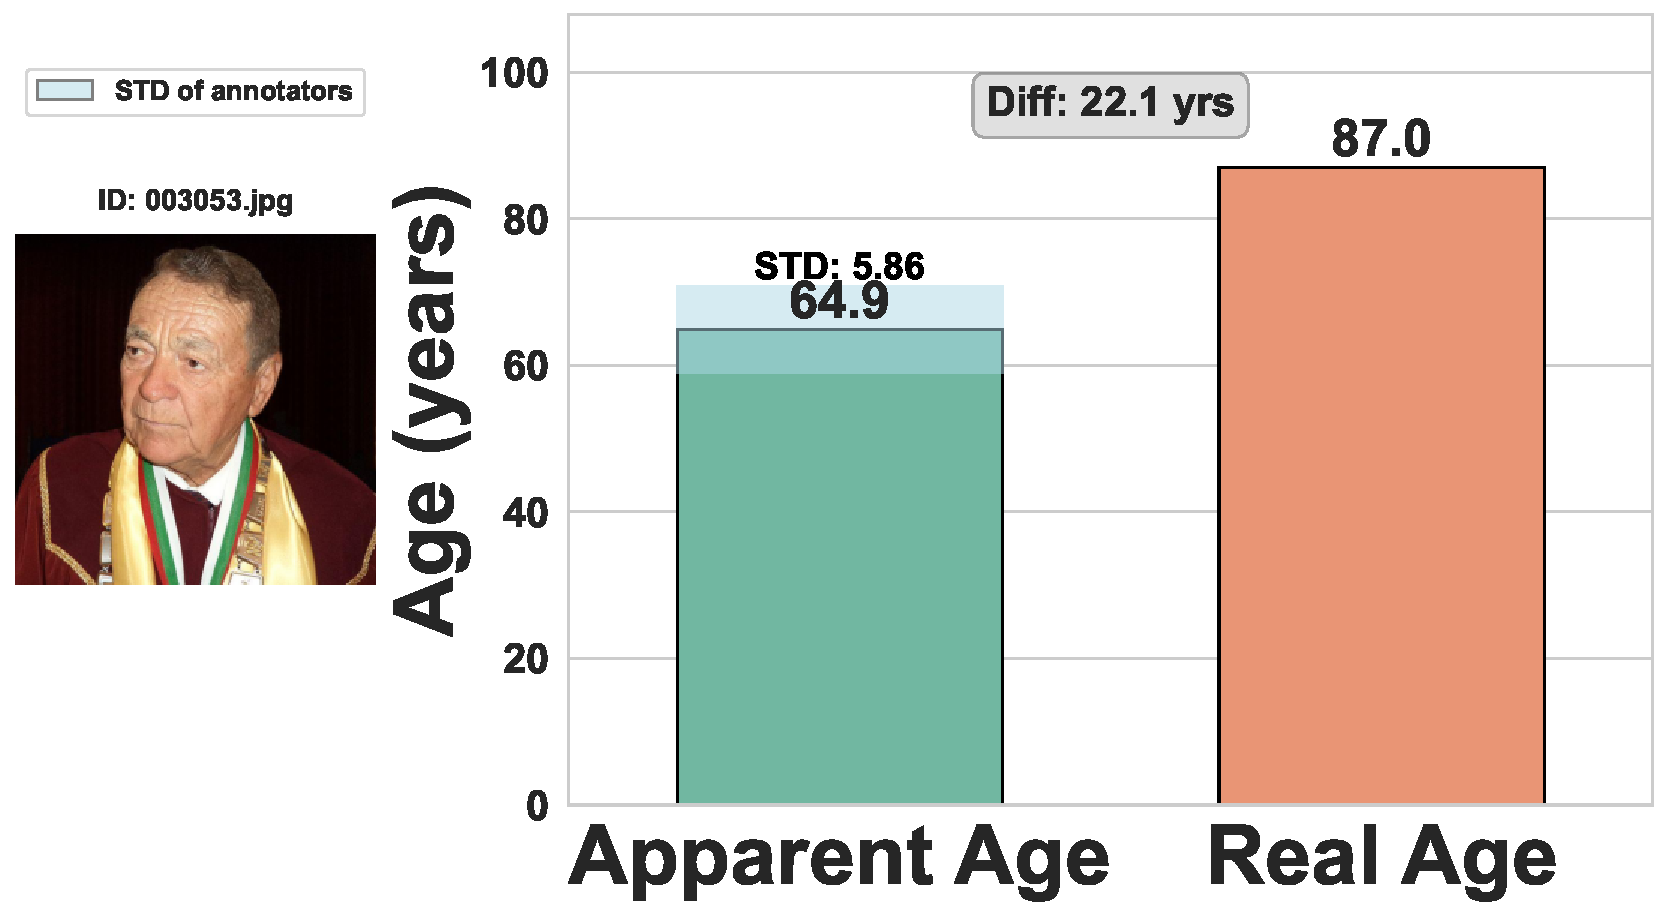
\includegraphics[width=\linewidth]{fig_elderly_example.pdf}
\caption{Elderly subject (ID:~003053). Real age 87, mean apparent label 64.9 (22.1-year underestimation).}
\end{subfigure}
\hfill
\begin{subfigure}[t]{0.48\linewidth}
\centering
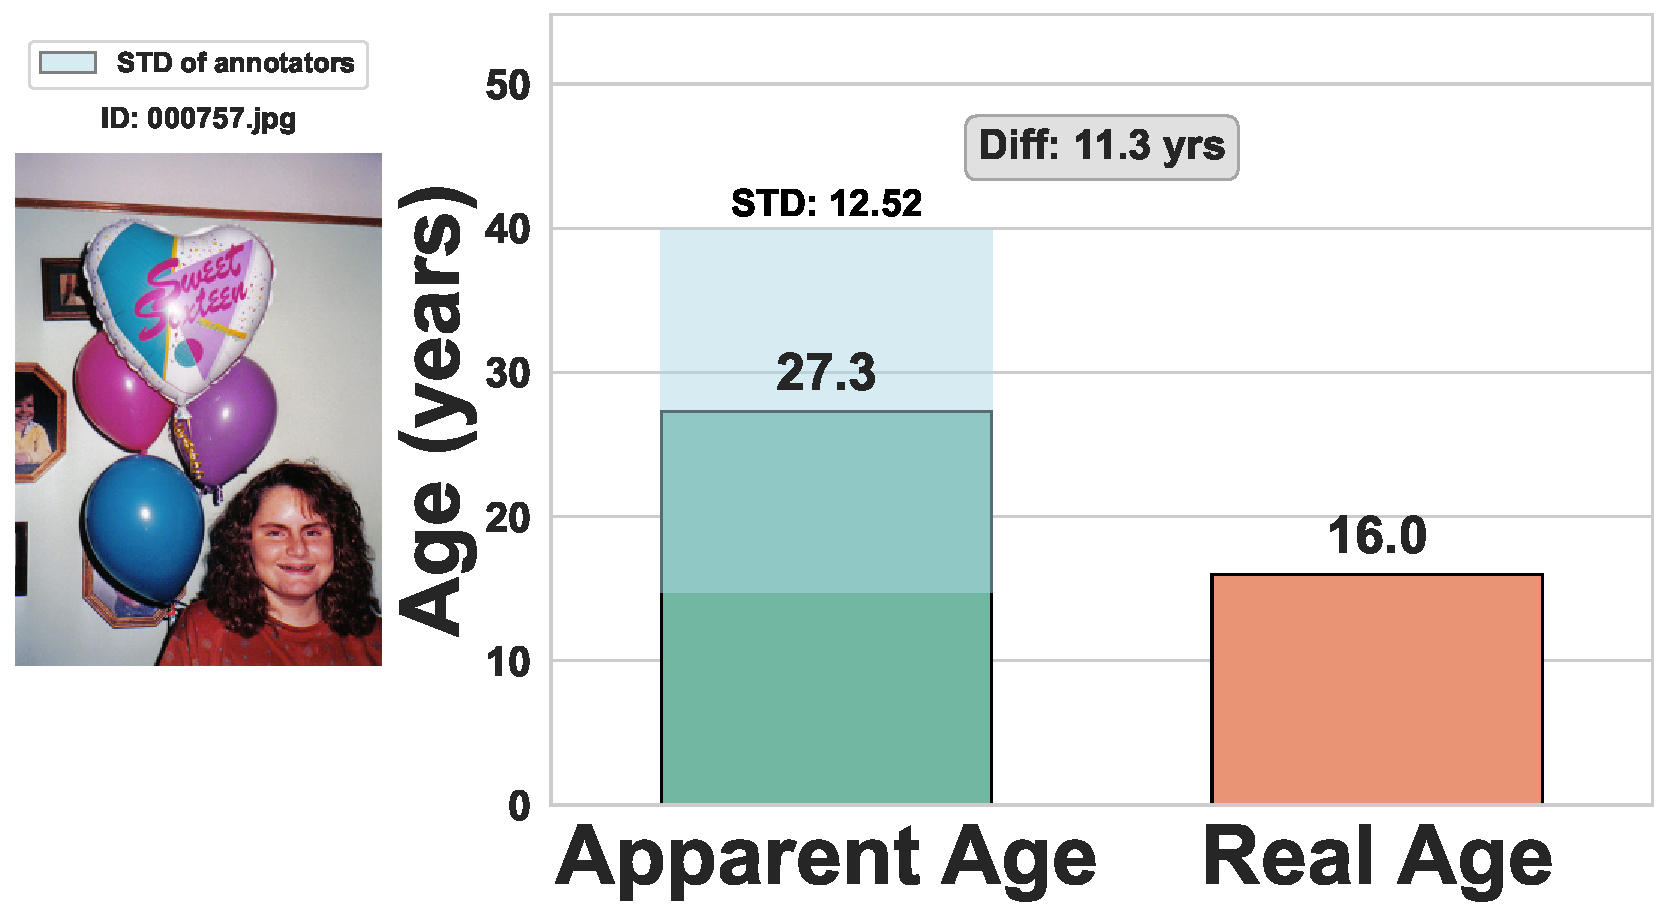
\includegraphics[width=\linewidth]{fig_young_example.pdf}
\caption{Young subject (ID:~000757). Real age 16, mean apparent label 27.3 (11.3-year overestimation).}
\end{subfigure}
\caption{Comparison of old (left) and young (right) apparent age estimation examples with uncertainty estimation. This paper proposes to learn human aleatoric uncertainty separately from epistemic uncertainty.}
\label{fig:examples}
\end{figure}

The ability to quantify and isolate each type of uncertainty has various applications. Out-of-distribution detection~\cite{henning2021bayesian} and Active Learning~\cite{lahlou2023deup} should isolate samples with high epistemic uncertainty, but should not be affected by aleatoric uncertainty. Aleatoric uncertainty can dominate in face age estimation due to larger inherent uncertainty, especially for older faces. In a decision-support system it can also be used to select different actions under different kinds of uncertainty~\cite{vangorp2022certainty}. If a human disagrees with a model that indicates high epistemic uncertainty, then the model may learn from the human annotation. If there is only aleatoric uncertainty, we might conclude that the human is overconfident in their age estimation.

While methods for disentangling these two types of uncertainty have been around for longer~\cite{kendall2017uncertainties,hullermeier2021aleatoric}, recent work has found that in classification contexts the two types of uncertainty are not successfully separated~\cite{mucsanyi2024benchmarking,wimmer2023quantifying,dejong2025measuring}. Since age estimation is a regression task, it is unknown whether these critiques on disentanglement apply or whether each uncertainty can be successfully isolated.

\subsection{Contributions}

We address the gap in a standard age prediction model by combining age regression with uncertainty quantification. Knowing only what a model predicts is insufficient; we must also understand how uncertain the model is, and why it is uncertain. And particularly in facial age estimation, there is a high degree of uncertainty, both coming from the model itself and labeling uncertainty, via the concept of apparent age, different humans will label face image with different age values, so a successful facial age estimation model must estimate both model and data uncertainties.

Previous work demonstrated that disentangling uncertainties is not effective in classification. We want to investigate whether these concerns extend to face age estimation. Therefore, this paper assesses how epistemic and aleatoric uncertainty estimates behave with respect to the size of the dataset on which a model is trained. This establishes whether epistemic uncertainty can be isolated in age estimation, despite the large amount of inherent aleatoric uncertainty.

We expect the aleatoric uncertainty to remain constant across the percentages of data, while the epistemic uncertainty should increase as the dataset size decreases.

This paper's contributions are:
\begin{itemize}
    \item A formulation of facial age regression with uncertainty estimation, producing separate estimates of model and data uncertainty.
    \item This formulation also learns from multiple human annotations (available in the APPA-REAL dataset), incorporating human uncertainty into the trained model. Our facial age estimation model outputs mean apparent age, apparent model uncertainty, and apparent data uncertainty (learned from human annotations).
    \item A cross-dataset evaluation on UTKFace that probes whether the learned uncertainty remains informative under distribution shift, complementing the in-distribution APPA-REAL results with calibration and qualitative analyses.
\end{itemize}

\section{Background}
\label{sec:background}

\subsection{Related Work}

Previous research on Uncertainty Quantification in face age estimation has been sparse, but showing some promising results. One approach has been to group ages into age-classes, so that age estimation can be treated as a classification problem~\cite{terhorst2019reliable}. This results models that produce age-class-probabilities, which can be used as a measure of uncertainty. Being selective in which classification gets used, based on a threshold on the class probability has been shown to improve age classification accuracy~\cite{terhorst2019reliable}. Mixture Density Networks have been applied on age estimation based on the IMDb-Wiki dataset~\cite{rothe2015dex}, but this dataset contains predominately Caucasian celebrities between 20 and 40 years old~\cite{terhorst2019reliable}.

Recent work by Mucs\'anyi et al.~\cite{mucsanyi2024benchmarking} provides a comprehensive empirical framework for evaluating how well current models can disentangle epistemic and aleatoric uncertainty in classification tasks. Their study reveals that standard methods often fail to achieve true disentanglement. This suggests that naive use of conventional Bayesian approximations may yield misleading uncertainty decompositions.

Unlike most prior work, which has focused on classification tasks, this paper applies these principles to a real-world regression problem: facial age estimation. We extend the classification-focused frameworks of prior studies by adapting their uncertainty estimation techniques: Monte Carlo Dropout, Flipout, and Deep Ensembles, for regression. These methods allow the model to output not only the mean prediction, the estimated apparent age, but also an associated variance, which serves as a measure of predictive uncertainty. To evaluate whether these uncertainties are disentangled in the regression setting, we replicate the experimental approach used in classification studies: we train models on different subset sizes of the dataset~\cite{dejong2025measuring}.

\subsection{Age Estimation From Faces}

Estimating a person's age from their facial image is a longstanding problem in computer vision. Age estimation can be used in security or access control; AI systems estimate age to restrict access to age-sensitive content, such as alcohol purchases or gambling~\cite{burgess2021ai}. Brands use age estimation to tailor content and ads based on the viewer's demographic profile~\cite{burt2023anonymized,gollapalli2023machine}.

Predicting a person's apparent age is especially difficult. Unlike biological age, apparent age is subjective and often biased~\cite{pilz2022contextual}, requiring models to approximate human perception. This makes it a more complex task than conventional regression~\cite{rothe2015dex}. Human perception of age is affected by systematic biases, such as the regression-to-the-mean effect, which causes younger individuals to be overestimated and older individuals to be underestimated in age estimation tasks~\cite{burt1995perception,clifford2018two}.

Additionally, external factors such as alcohol and tobacco consumption can significantly affect perceived age. Studies have shown that heavy drinking and smoking accelerate visible facial aging, making individuals appear older than their biological age~\cite{goodman2019impact}.

Another challenge arises from the visual similarity within specific age ranges. Older adults, between 60 and 80 years old, tend to have less distinctive facial features that differentiate their precise age, leading to higher estimation errors~\cite{ganel2023biases}. Similarly, prepubescent children, under 13, display subtle differences in facial features that make age estimation in this group particularly difficult~\cite{ferguson2017juvenile}.

Despite these systematic tendencies to underestimate older adults and overestimate children, quantifying exactly how large those deviations can become is crucial. To illustrate this, we present two representative subjects whose apparent-age labels diverge significantly from their actual ages. Figures~\ref{fig:examples}(a) and~\ref{fig:examples}(b) respectively show an 87-year-old and a 16-year-old, each annotated by the same group of raters. These examples highlight the scale and direction of human perceptual bias.

Figure~\ref{fig:examples}(a) presents an elderly subject with an actual chronological age of 87 years. Human annotators provided an average apparent age label of 64.9 years, underestimating their actual age by 22.1 years. Facial features, such as fine wrinkles, skin texture, and hair color, can be interpreted variably, leading to significant variance in labeling.

Conversely, Figure~\ref{fig:examples}(b) shows a youthful subject aged 16 years. The same group of annotators assigned an average apparent age of 27.3 years, overestimating by 11.3 years. This overestimation reveals how youthful faces can be biased upward when compared against adult-centric benchmarks.

\subsection{Uncertainty Estimation}

In regression problems, we can treat model and data uncertainty as variances, and have the total predictive variance $\sigma^2_{\mathrm{pred}}(\cdot)$ for some input $x^*$ as
\begin{equation}
\sigma^2_{\mathrm{pred}}(x^*) = \underbrace{\mathbb{E}\!\left[\sigma^2_{\mathrm{aleatoric}}(x^*)\right]}_{\text{Aleatoric uncertainty}} + \underbrace{\mathrm{Var}\!\left[\mu(x^*)\right]}_{\text{Epistemic uncertainty}}.
\label{eq:total}
\end{equation}
The disentanglement of the uncertainties is the separation of these two aforementioned uncertainties.

Aleatoric uncertainty is inherent uncertainty in the data. In apparent age estimation, it arises from annotator disagreement. Mathematically, aleatoric uncertainty is expressed as the variance of the output. This is written as:
\begin{equation}
\sigma^2_{\mathrm{aleatoric}}(x) = \mathrm{Var}[y\mid x].
\label{eq:aleatoric}
\end{equation}
Here, $\mathrm{Var}[y\mid x]$ denotes the conditional variance of the output given a particular input. In this study, the variance is learned alongside the prediction of the mean, enabling the model to express confidence in its outputs by explicitly estimating the aleatoric uncertainty.

On the other hand, epistemic uncertainty arises not from the data itself but from the limitations of the model. It can be caused by various problems, including small datasets, class imbalance, overfitting, underfitting, or, more broadly, the model failing to generalize. In Bayesian models, epistemic uncertainty is estimated by evaluating the extent to which the model's predictions vary across different parameter configurations. This idea is captured in the following formula:
\begin{equation}
\mathrm{Var}[\mu(x)] = \frac{1}{T}\sum_{t=1}^{T}\mu_t^2(x) - \left(\frac{1}{T}\sum_{t=1}^{T}\mu_t(x)\right)^2.
\label{eq:epistemic}
\end{equation}
Here, the model is run $T$ times for the same input $x$, each time with different dropout configurations, resulting in different predicted means $\mu_t(x)$. The first term, $\tfrac{1}{T}\sum_{t=1}^{T}\mu_t^2(x)$, is the average of the squared predictions, and the second term, $\bigl(\tfrac{1}{T}\sum_{t=1}^{T}\mu_t(x)\bigr)^2$, is the square of the average prediction. Their difference yields the variance of the predictions, which quantifies the model's uncertainty about its output.

\section{Facial Age Estimation with Uncertainty}
\label{sec:method}

\paragraph{Dataset.}
This study uses the APPA-REAL dataset~\cite{agustsson2017appareal}, which contains 7,591 images annotated with both real age and apparent age. Apparent age labels are obtained from human perception studies: each image was rated by multiple annotators, and the final apparent age corresponds to the mean of all votes. In total, the dataset comprises approximately 250,000 individual annotations, with an average of 38 votes per image, resulting in a low standard error of the mean of 0.3.

In addition to the mean apparent age, each image is annotated with the standard deviation of the votes, which reflects annotator disagreement and provides a measure of uncertainty. This enables the modeling of both the expected apparent age and its associated uncertainty.

Each subject is represented by two image types: full-body images including contextual information, and cropped facial images. Facial images are extracted and aligned using the face detection method described in~\cite{mathias2014face}, with a 40\% margin around the detected face and support for multiple orientations. Only facial images are used in this work. Each image is accompanied by a MATLAB file containing face-related metadata.

The dataset is split into 4,113 training images, 1,500 validation images, and 1,978 test images. The training set exhibits a strong class imbalance, with a high concentration of samples in the 20--40 age range (Fig.~\ref{fig:appa_distrib}). The Pearson correlation coefficient between real age and apparent age is 0.94, indicating a strong relationship between the two variables (Fig.~\ref{fig:appa_scatter}). While the maximum observed error exceeds 25 years, most errors are below 10 years and follow an approximately normal distribution (Fig.~\ref{fig:appa_error}).

\begin{figure}[t]
\centering
\begin{subfigure}[t]{0.32\linewidth}
\centering
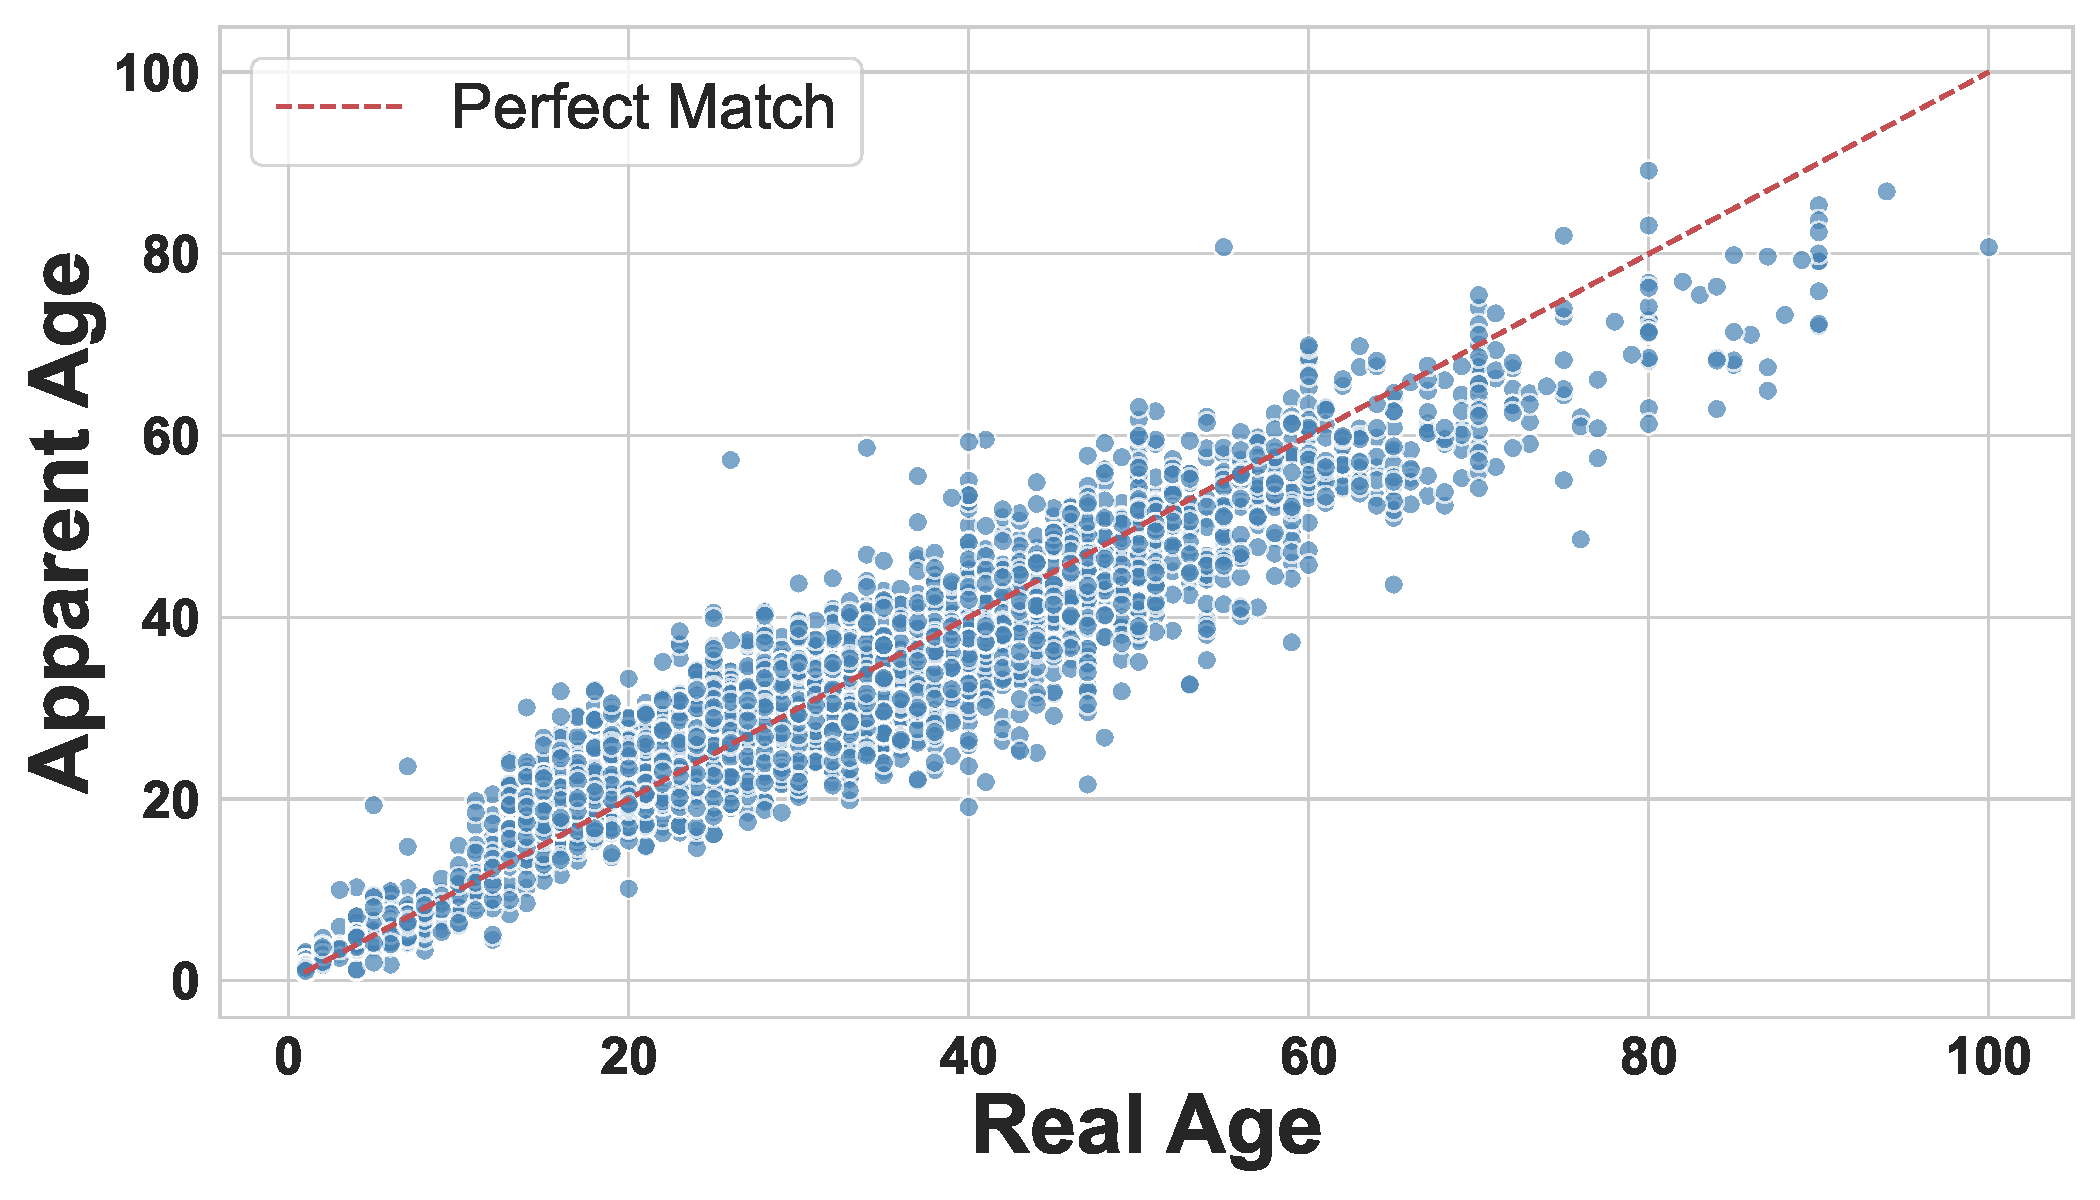
\includegraphics[width=\linewidth]{fig_scatter.pdf}
\caption{Scatterplot.}
\label{fig:appa_scatter}
\end{subfigure}
\hfill
\begin{subfigure}[t]{0.32\linewidth}
\centering
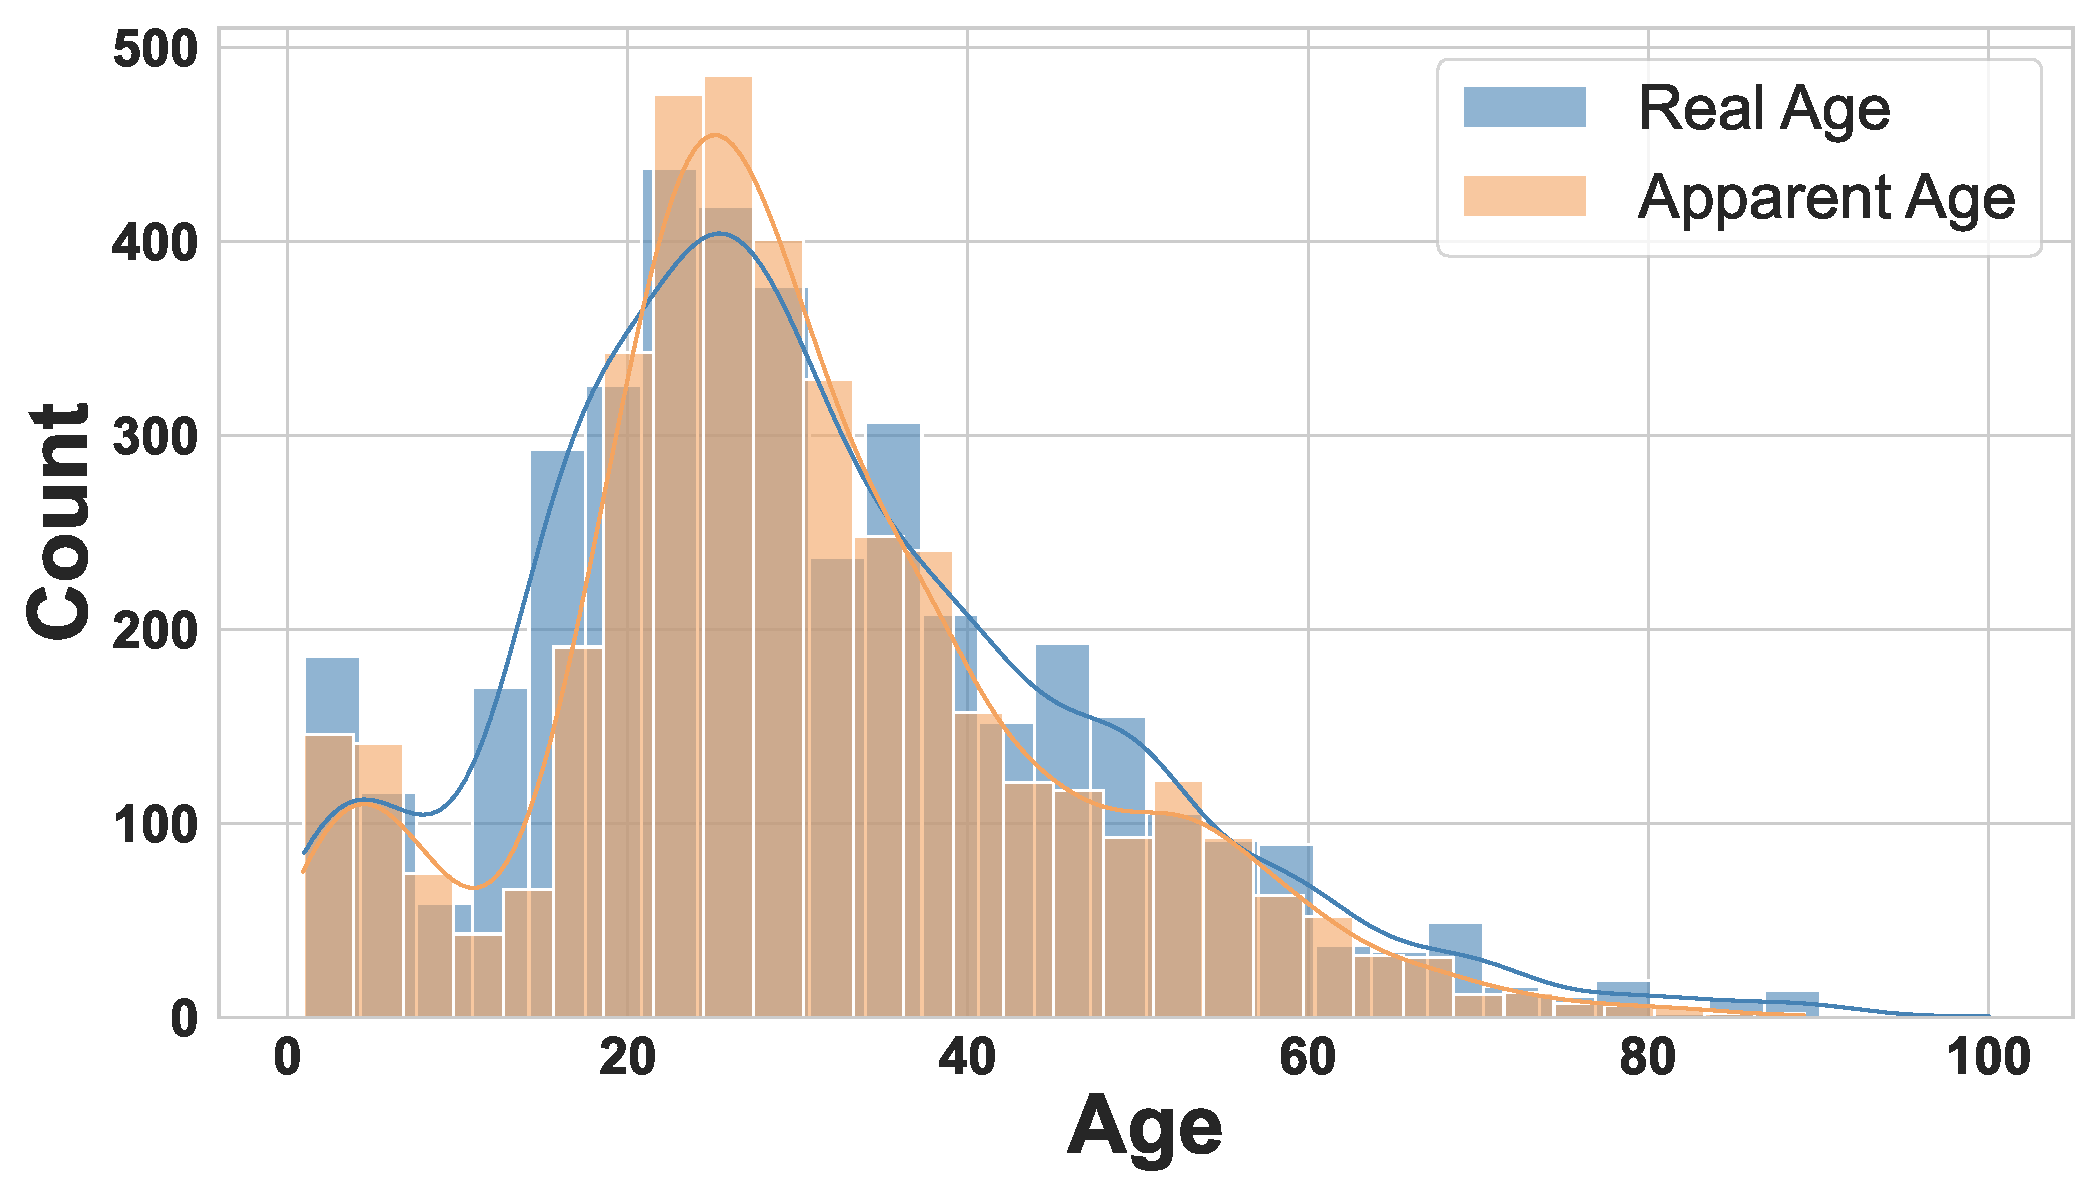
\includegraphics[width=\linewidth]{fig_age_distribution.pdf}
\caption{Age distribution.}
\label{fig:appa_distrib}
\end{subfigure}
\hfill
\begin{subfigure}[t]{0.32\linewidth}
\centering
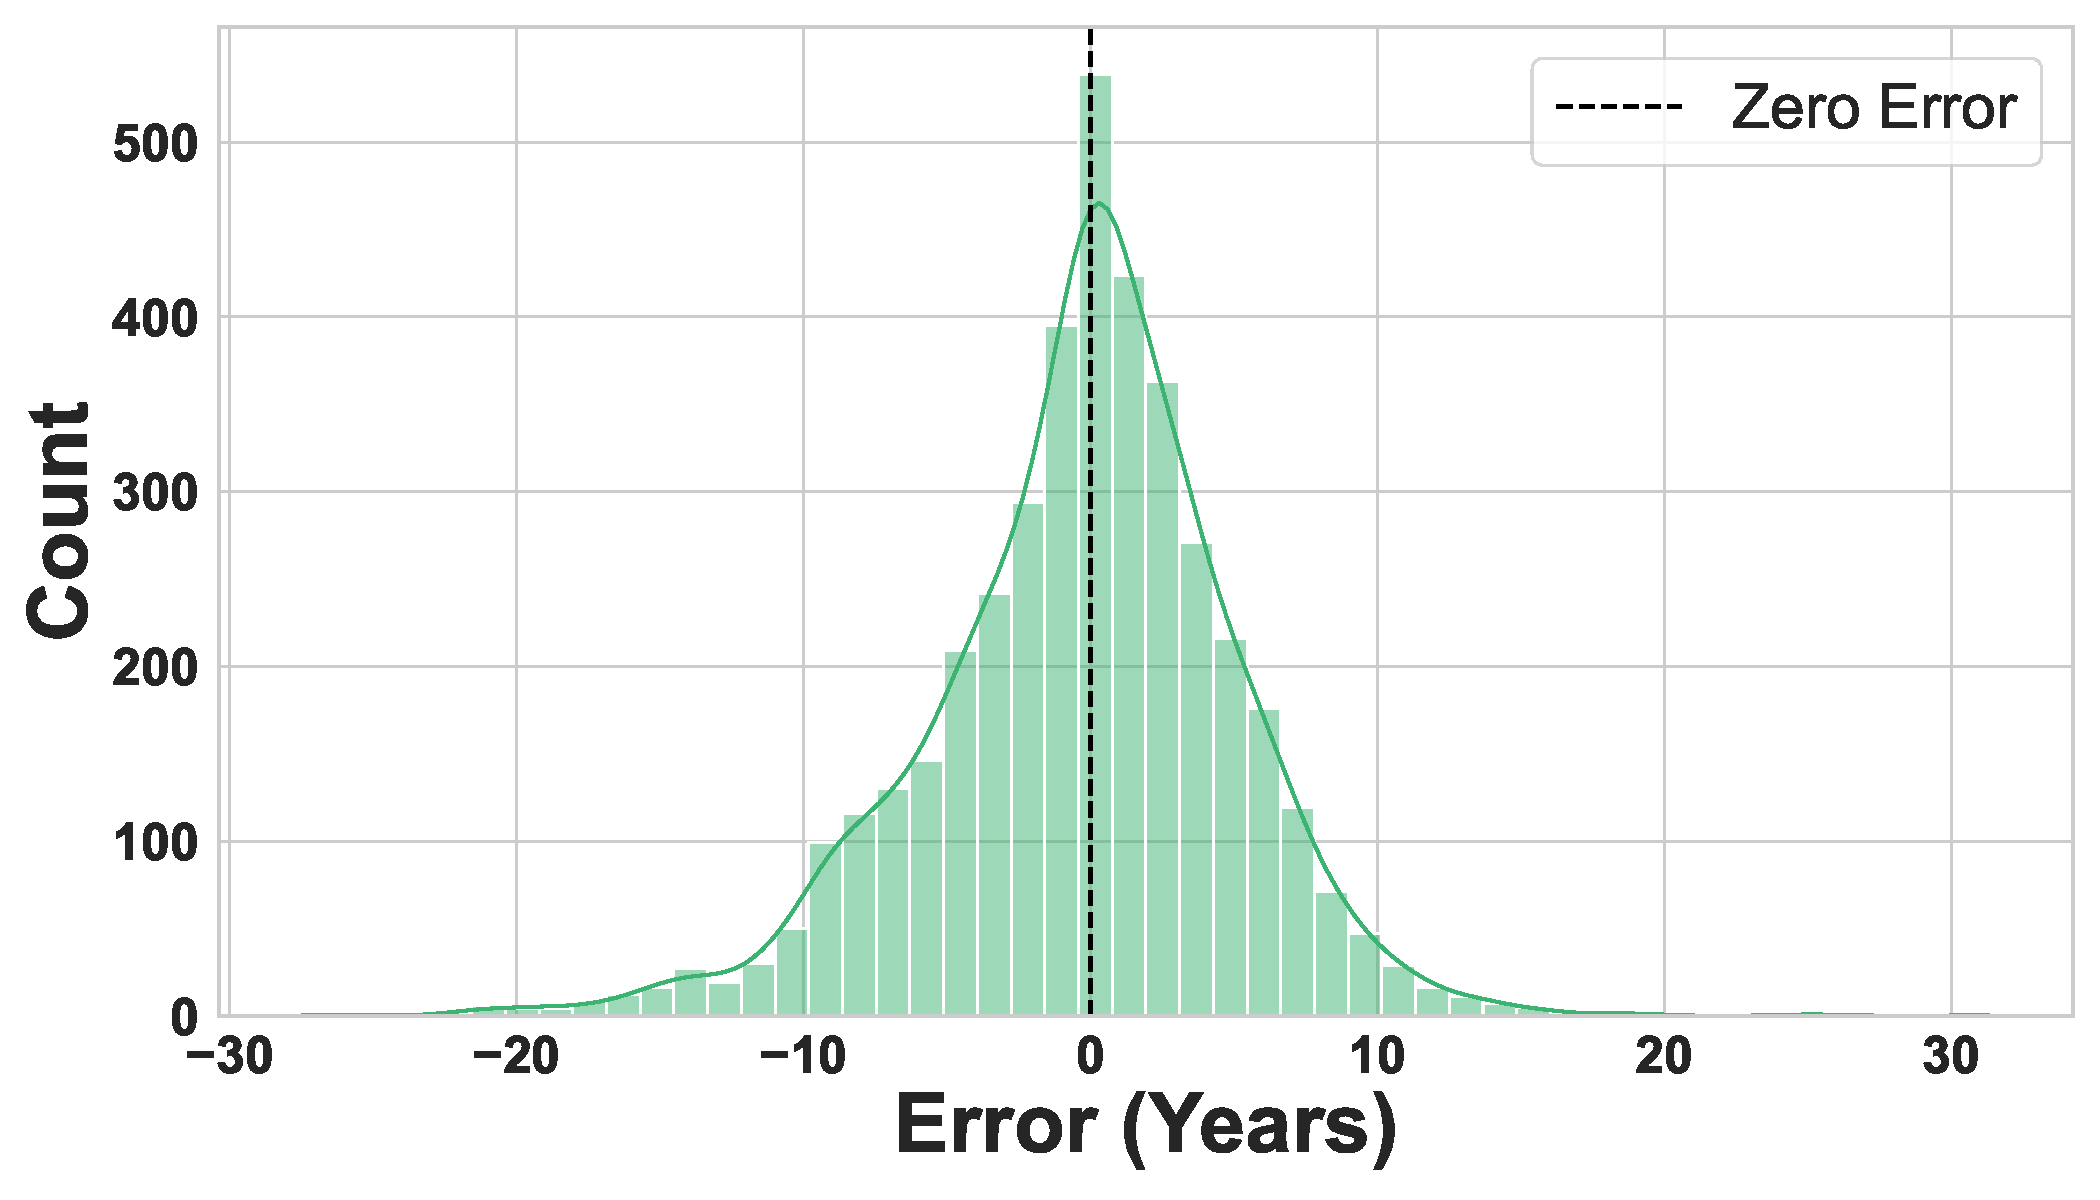
\includegraphics[width=\linewidth]{fig_age_error.pdf}
\caption{Age error (Apparent$-$Real).}
\label{fig:appa_error}
\end{subfigure}
\caption{Distribution of real and apparent age in the APPA-REAL dataset. On average, the apparent age matches the real age quite well, except for an increased uncertainty.}
\label{fig:appa}
\end{figure}

\paragraph{Preprocessing.}
A custom data loading and preprocessing pipeline was implemented using TensorFlow and Keras to ensure consistency across experiments and efficient training. Since models are trained on varying proportions of the dataset, a stratified subsampling strategy is employed to preserve the original label distribution across subsets.

To achieve this, apparent age labels are discretized using quantile binning, allowing uniform sampling across bins while maintaining proportional age-group representation. Images are resized to $224 \times 224$ pixels using Keras utilities. Data augmentation is applied to improve robustness and reduce overfitting, including random rotations ($\pm 10^{\circ}$), horizontal and vertical shifts (up to 10\%), zooming (80--120\%), horizontal flipping, and brightness variation (80--120\%). For each sample, a random augmentation strategy is applied, followed by normalization.

\paragraph{Model architecture.}
The proposed model is a multi-output regression architecture that jointly predicts the mean apparent age and its standard deviation. The backbone is a DenseNet-121 network~\cite{huang2017densely} pre-trained on ImageNet~\cite{deng2009imagenet}, selected for its efficient feature reuse and strong gradient propagation.

Extracted features are passed to a shared regression head consisting of two fully connected layers with 512 and 256 neurons. Each layer is followed by batch normalization and Leaky ReLU activation. L2 regularization is applied to dense weights, and a dropout layer with a rate of 0.5 is used after the shared layers to improve generalization.

The network then branches into two outputs. The mean apparent age branch uses a 128-neuron dense layer with ReLU activation followed by a single-neuron ReLU output to enforce non-negative predictions. The uncertainty branch mirrors this structure but uses a Softplus activation in the final layer to ensure strictly positive standard deviation estimates.

\paragraph{Training setup.}
We implemented a comprehensive training pipeline structured in three distinct phases: initial single-task training, multitask training, and fine-tuning. This phased approach follows principles similar to curriculum learning and staged training~\cite{bengio2009curriculum,howard2018universal}, enabling progressive learning. While our primary motivation for multitask learning is uncertainty quantification, prior work suggests that multitask setups can also enhance generalization and convergence behavior~\cite{caruana1997multitask}.

The model produces two outputs per image: mean apparent age and apparent age uncertainty, expressed as a standard deviation. Crucially, the uncertainty branch is explicitly supervised. The APPA-REAL dataset provides multiple human annotations per image; from these annotations, we compute the mean apparent age, used as the regression target for the mean branch, and the standard deviation of human votes, which reflects annotator disagreement and serves as a proxy for aleatoric uncertainty. This preprocessing step yields a per-image uncertainty target that allows the model to learn how uncertain humans are about a given face, rather than inferring aleatoric uncertainty indirectly.

In the first phase, only the mean age branch is trained using Mean Squared Error (MSE) loss, while the uncertainty branch is disabled via a zero-weighted dummy loss. In the second phase, both branches are jointly optimized using MSE, and most DenseNet layers are unfrozen to allow task-specific feature adaptation. In the final phase, all backbone layers are unfrozen to enable fine-grained tuning across the entire network.

The Adam optimizer is used throughout training with a learning rate of $2 \times 10^{-4}$, which is reduced to $1 \times 10^{-5}$ during fine-tuning.

To ensure fair training across dataset sizes, a dynamic epoch allocation strategy is employed, following~\cite{dejong2025measuring}. For the first two phases, the maximum number of epochs is scaled inversely with the fraction of training data, using a base of 100 epochs. For example, training with 1\% of the data allows up to 10,000 epochs, while using 100\% allows 100 epochs. The fine-tuning phase uses 25\% of the allocated epochs. This strategy normalizes the total number of optimization steps across dataset sizes.

Early stopping is applied in all phases to prevent overfitting, with patience values of 5, 7, and 10 epochs for the first, second, and third phases, respectively.

\paragraph{Uncertainty disentanglement.}
To disentangle aleatoric and epistemic uncertainty, four methods are evaluated: MC-Dropout~\cite{gal2016dropout}, MC-DropConnect~\cite{mobiny2021dropconnect}, Flipout~\cite{wen2018flipout}, and Deep Ensembles~\cite{lakshminarayanan2017simple}. These approaches are inspired by Bayesian Neural Networks (BNNs), which model uncertainty by placing distributions over network weights~\cite{blundell2015weight}. Although exact Bayesian inference is intractable for deep networks, approximate methods enable practical uncertainty estimation~\cite{kendall2017uncertainties}.

In this study, the final dense layers are replaced with stochastic variants. MC-Dropout~\cite{gal2016dropout} keeps dropout active during inference, allowing multiple stochastic forward passes to approximate posterior sampling. MC-DropConnect~\cite{wan2013regularization} instead applies stochastic masks to weights, with a drop rate of 0.3. Flipout~\cite{wen2018flipout} introduces pseudo-independent weight perturbations per input, reducing gradient variance and improving training stability. Deep Ensembles~\cite{lakshminarayanan2017simple} estimate uncertainty by training multiple independently initialized models and interpreting their diversity as epistemic uncertainty.

Aleatoric uncertainty is computed as the mean predicted variance across forward passes, while epistemic uncertainty is estimated as the variance of the predicted means.

\paragraph{Experimental setup.}
To find how the epistemic and aleatoric uncertainty behave with respect to dataset size, we trained the models on seven different percentages of the dataset. These percentages are: 1\%, 5\%, 10\%, 25\%, 50\%, 75\%, 100\%; they were chosen based on the study by~\cite{dejong2025measuring}. Each subset has the same distribution of the labels, so the only difference between the subsets is the number of samples. For example, the smallest subset (1\% of the training set) has only 40 samples.

Each type of model is trained using the specified percentages of the data and then inferred through twenty forward passes.

\section{Results}
\label{sec:results}

We begin by examining how predictive uncertainty evolves as a function of training dataset size, followed by a method-specific analysis of uncertainty behavior. We then evaluate predictive performance using standard regression metrics (MAE, RMSE, and $R^2$) and relate accuracy trends to uncertainty estimates. We highlight notable anomalies observed during experimentation, and conclude with a cross-dataset evaluation on UTKFace.

Table~\ref{tab:unc} and Fig.~\ref{fig:unc} summarize the estimated aleatoric and epistemic uncertainties across different training data percentages for the three uncertainty estimation methods.

Across all methods, aleatoric uncertainty remains largely stable as dataset size increases, while epistemic uncertainty generally decreases. For instance, in the DropConnect method, epistemic uncertainty drops from 12.89 years squared at 5\% of the data to 6.05 years squared at full data. Similar decreasing trends are observed for the other methods, albeit with different magnitudes. In contrast, aleatoric uncertainty consistently remains around 18--19 years squared, with only minor fluctuations.

These results support the central hypothesis of this paper: epistemic uncertainty is inversely related to data volume, whereas aleatoric uncertainty remains approximately constant.

\begin{table}[t]
\centering
\caption{Aleatoric and epistemic uncertainty by model and training-data percentage.}
\label{tab:unc}
\begin{tabular}{rcccccc}
\toprule
& \multicolumn{2}{c}{DROPCONNECT} & \multicolumn{2}{c}{ENSEMBLE} & \multicolumn{2}{c}{FLIPOUT} \\
\cmidrule(lr){2-3}\cmidrule(lr){4-5}\cmidrule(lr){6-7}
Training data (\%) & Aleatoric & Epistemic & Aleatoric & Epistemic & Aleatoric & Epistemic \\
\midrule
1   & 1.340  & 12.251 & 2.018  & 1.923 & 8.364  & 2.433 \\
5   & 19.855 & 12.891 & 13.902 & 1.862 & 2.404  & 7.072 \\
10  & 18.668 & 12.019 & 18.741 & 1.815 & 18.434 & 8.725 \\
25  & 18.286 & 10.890 & 18.601 & 1.783 & 17.655 & 8.994 \\
50  & 19.243 & 7.472  & 18.707 & 1.655 & 18.375 & 8.764 \\
75  & 18.865 & 6.006  & 18.890 & 1.600 & 18.499 & 8.536 \\
100 & 18.838 & 6.054  & 18.870 & 1.498 & 18.144 & 8.176 \\
\bottomrule
\end{tabular}
\end{table}

\begin{figure}[t]
\centering
\begin{subfigure}[t]{0.32\linewidth}
\centering
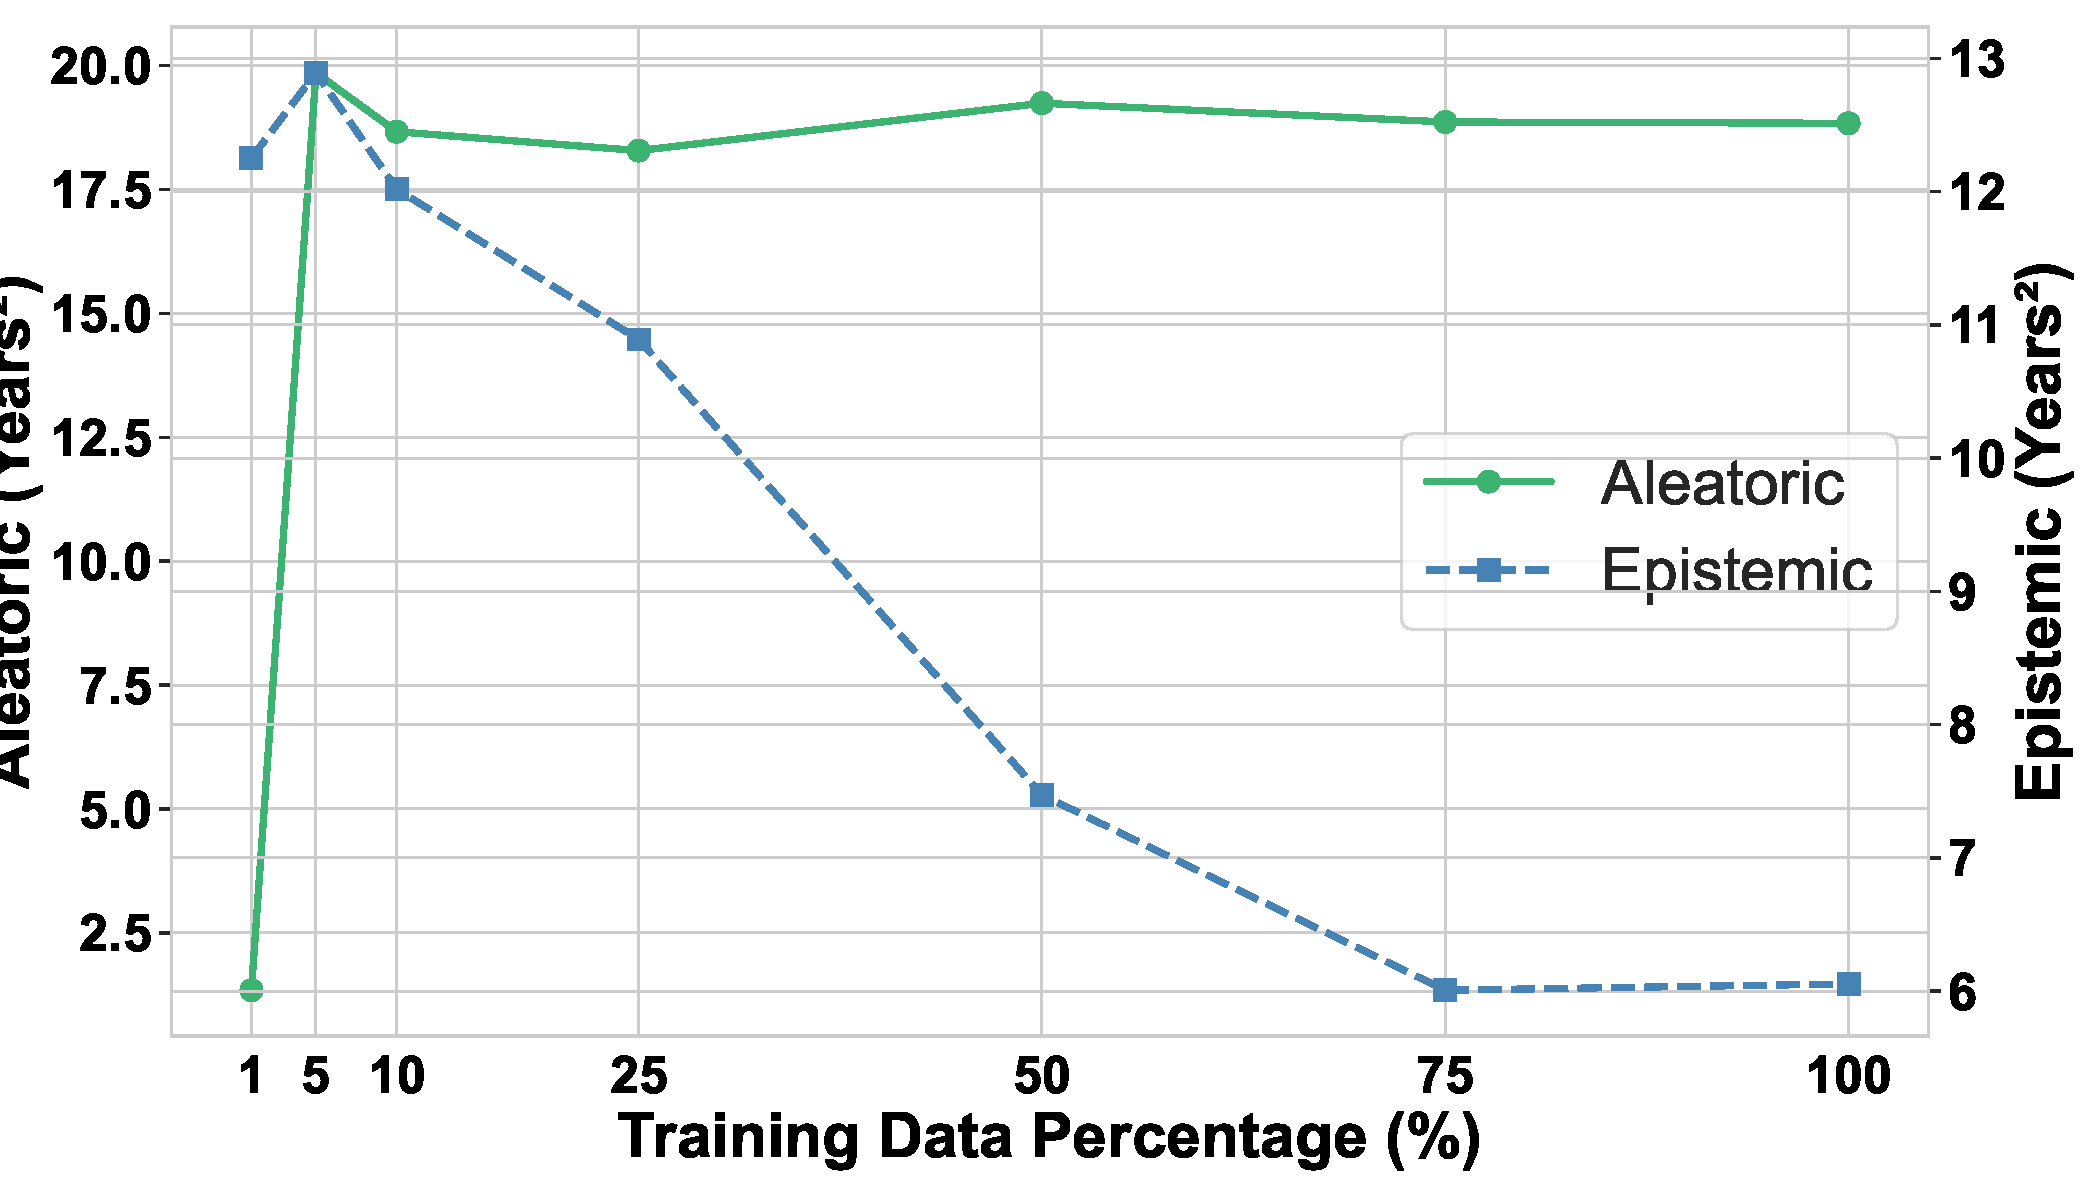
\includegraphics[width=\linewidth]{fig_unc_dropconnect.pdf}
\caption{DropConnect.}
\end{subfigure}
\hfill
\begin{subfigure}[t]{0.32\linewidth}
\centering
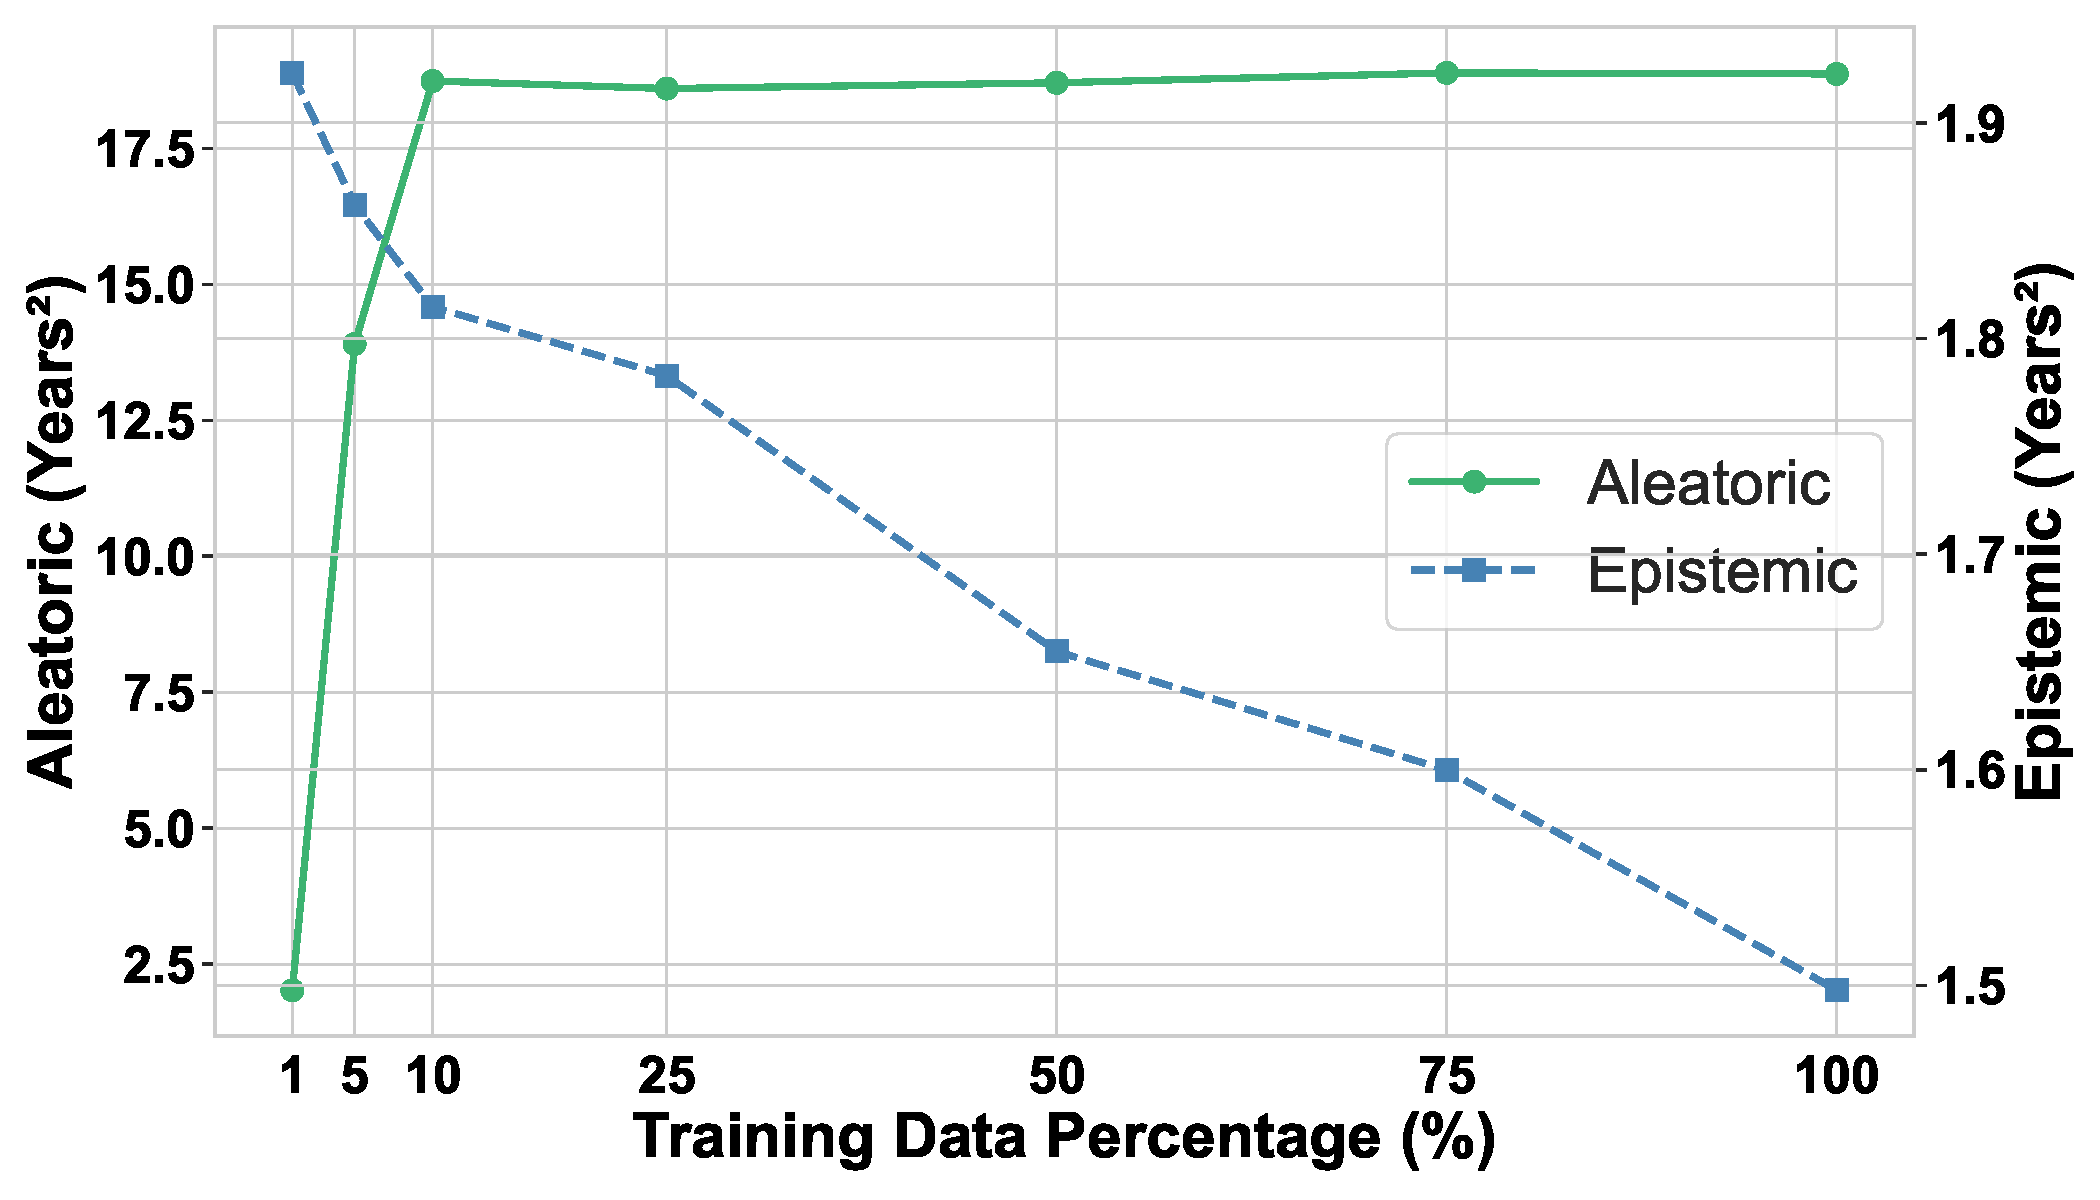
\includegraphics[width=\linewidth]{fig_unc_ensemble.pdf}
\caption{Ensembles.}
\end{subfigure}
\hfill
\begin{subfigure}[t]{0.32\linewidth}
\centering
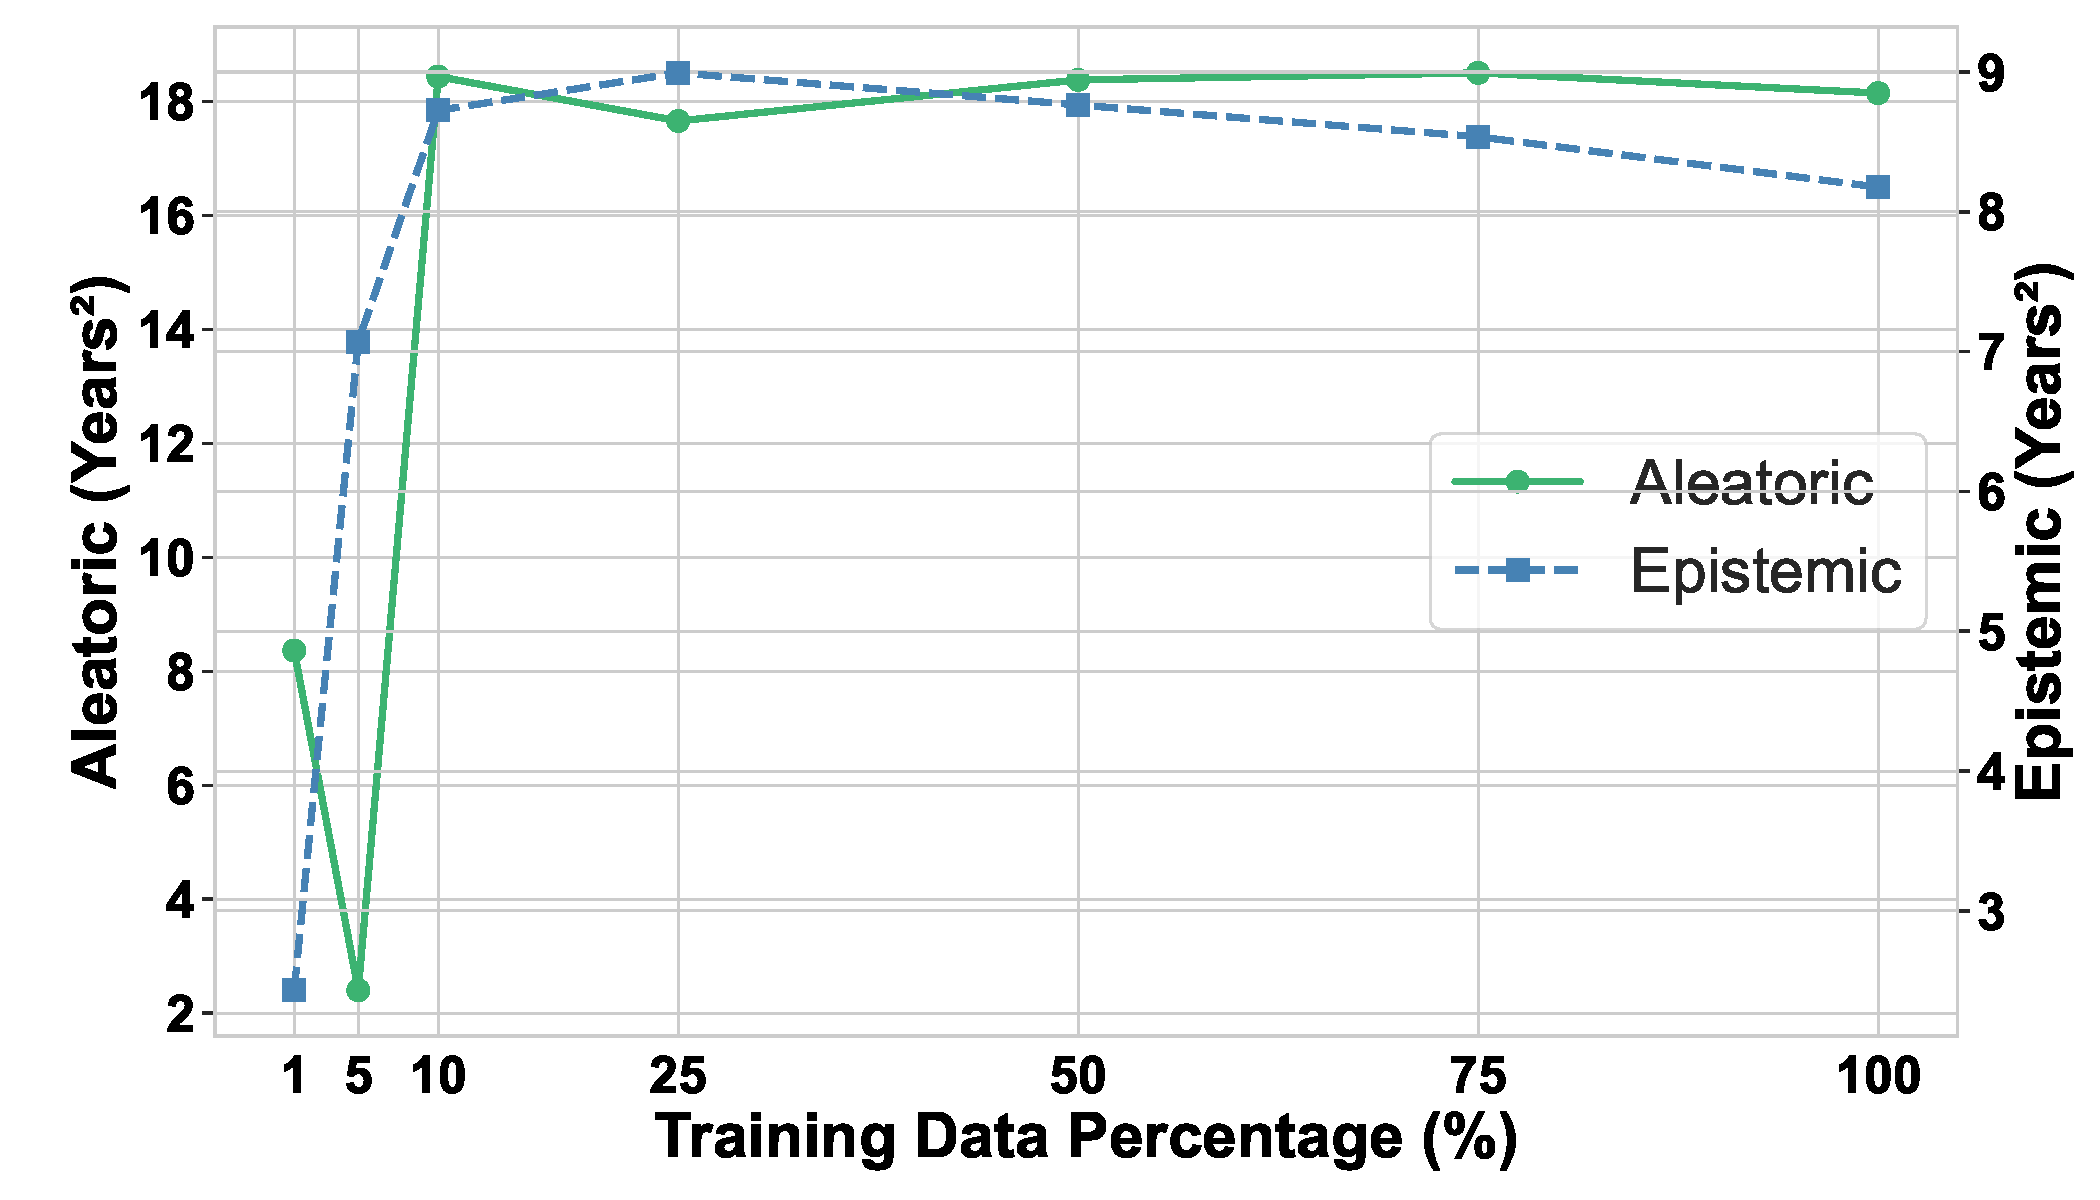
\includegraphics[width=\linewidth]{fig_unc_flipout.pdf}
\caption{Flipout.}
\end{subfigure}
\caption{Uncertainty trends using several uncertainty estimation methods across different training data percentages.}
\label{fig:unc}
\end{figure}

\subsection{Uncertainty Trends Across Dataset Sizes}

We analyze uncertainty behavior for three methods: DropConnect, Deep Ensembles, and Flipout. Table~\ref{tab:unc} reports the corresponding aleatoric and epistemic uncertainties for training data percentages ranging from 1\% to 100\%. Training on 1\% of the dataset corresponds to approximately 40 samples and resulted in severe underfitting. Consequently, uncertainty estimates at this level are unreliable and excluded from interpretation.

Uncertainty values are reported as variances of the predicted apparent age, measured in years squared. Although aleatoric values around 18 may appear high, they represent squared deviations; taking the square root yields a standard deviation of approximately 4.2 years.

Across all meaningful dataset sizes, aleatoric uncertainty remains stable at approximately 18 years squared, reinforcing its data-inherent nature. In contrast, epistemic uncertainty is consistently lower at 100\% training data than at smaller data fractions, with the steepest decline observed for DropConnect.

\paragraph{DropConnect.}
Fig.~\ref{fig:unc}(a) illustrates the response of DropConnect to increasing training data. This method exhibits the most pronounced reduction in epistemic uncertainty, decreasing from 12.89 years squared at 5\% of the data to 6.05 years squared at full data, a reduction of approximately 53\%. From 10\% onward, epistemic uncertainty decreases monotonically (12.02, 10.89, 7.47, and finally 6.05 years squared), indicating strong sensitivity to data availability. Aleatoric uncertainty remains stable for DropConnect, fluctuating only between 18.2 and 19.8 years squared from 10\% to 100\% of the data.

\paragraph{Deep Ensemble.}
Fig.~\ref{fig:unc}(b) shows that Deep Ensembles maintain consistently low epistemic uncertainty across all dataset sizes, decreasing slightly from 1.862 years squared at 5\% to 1.498 years squared at 100\%. The limited variation (less than 0.5 years squared) suggests that ensembles are less sensitive to dataset size, likely due to robustness arising from model diversity. Aleatoric uncertainty remains stable and comparable to other methods, hovering around 18.8 years squared from 10\% data onward. While this behavior confirms the data-inherent nature of aleatoric uncertainty, the consistently low epistemic values may indicate that ensembles underestimate model uncertainty in low-data regimes or benefit from strong implicit regularization.

\paragraph{Flipout.}
Fig.~\ref{fig:unc}(c) presents a distinct uncertainty profile for Flipout. Epistemic uncertainty decreases from 8.725 years squared at 10\% to 8.176 years squared at 100\%, but the decline is more gradual and less consistent than for DropConnect. Notably, epistemic uncertainty increases slightly between 10\% and 25\% of the data before decreasing again, suggesting instability in the variational approximation or sensitivity to training dynamics. Despite this noise, the overall trend aligns with theoretical expectations. Aleatoric uncertainty remains high and stable from 10\% data onward (17.6--18.5 years squared), further confirming its independence from dataset size.

\subsection{Prediction Accuracy Across Dataset Sizes}

In addition to uncertainty estimation, we evaluate predictive accuracy using MAE, RMSE, and $R^2$ across all dataset sizes and methods.

Fig.~\ref{fig:metrics}(a) shows that MAE decreases steadily with increasing data for all methods. DropConnect reduces its MAE from over 11.2 years at 5\% data to 8.3 years at full data. Deep Ensembles achieve the best overall performance with a final MAE of 8.0 years, while Flipout converges more slowly, reaching 8.9 years at 100\%.

Fig.~\ref{fig:metrics}(b) reveals similar trends. Deep Ensembles consistently outperform the other methods, followed by DropConnect and then Flipout. The monotonic reduction in RMSE highlights increasing prediction precision with larger datasets.

The relative performance is further illustrated in Fig.~\ref{fig:metrics}(c). At full data, Deep Ensembles achieve an $R^2$ score of 0.61, followed by DropConnect at 0.58 and Flipout at 0.53. These results confirm that predictive accuracy improves alongside increasing data availability.

Overall, all models benefit from larger training datasets, but Deep Ensembles provide the strongest raw predictive performance. Importantly, improvements in accuracy are accompanied by reductions in epistemic uncertainty, indicating that increased confidence coincides with improved prediction quality as data availability grows.

\begin{figure}[t]
\centering
\begin{subfigure}[t]{0.32\linewidth}
\centering
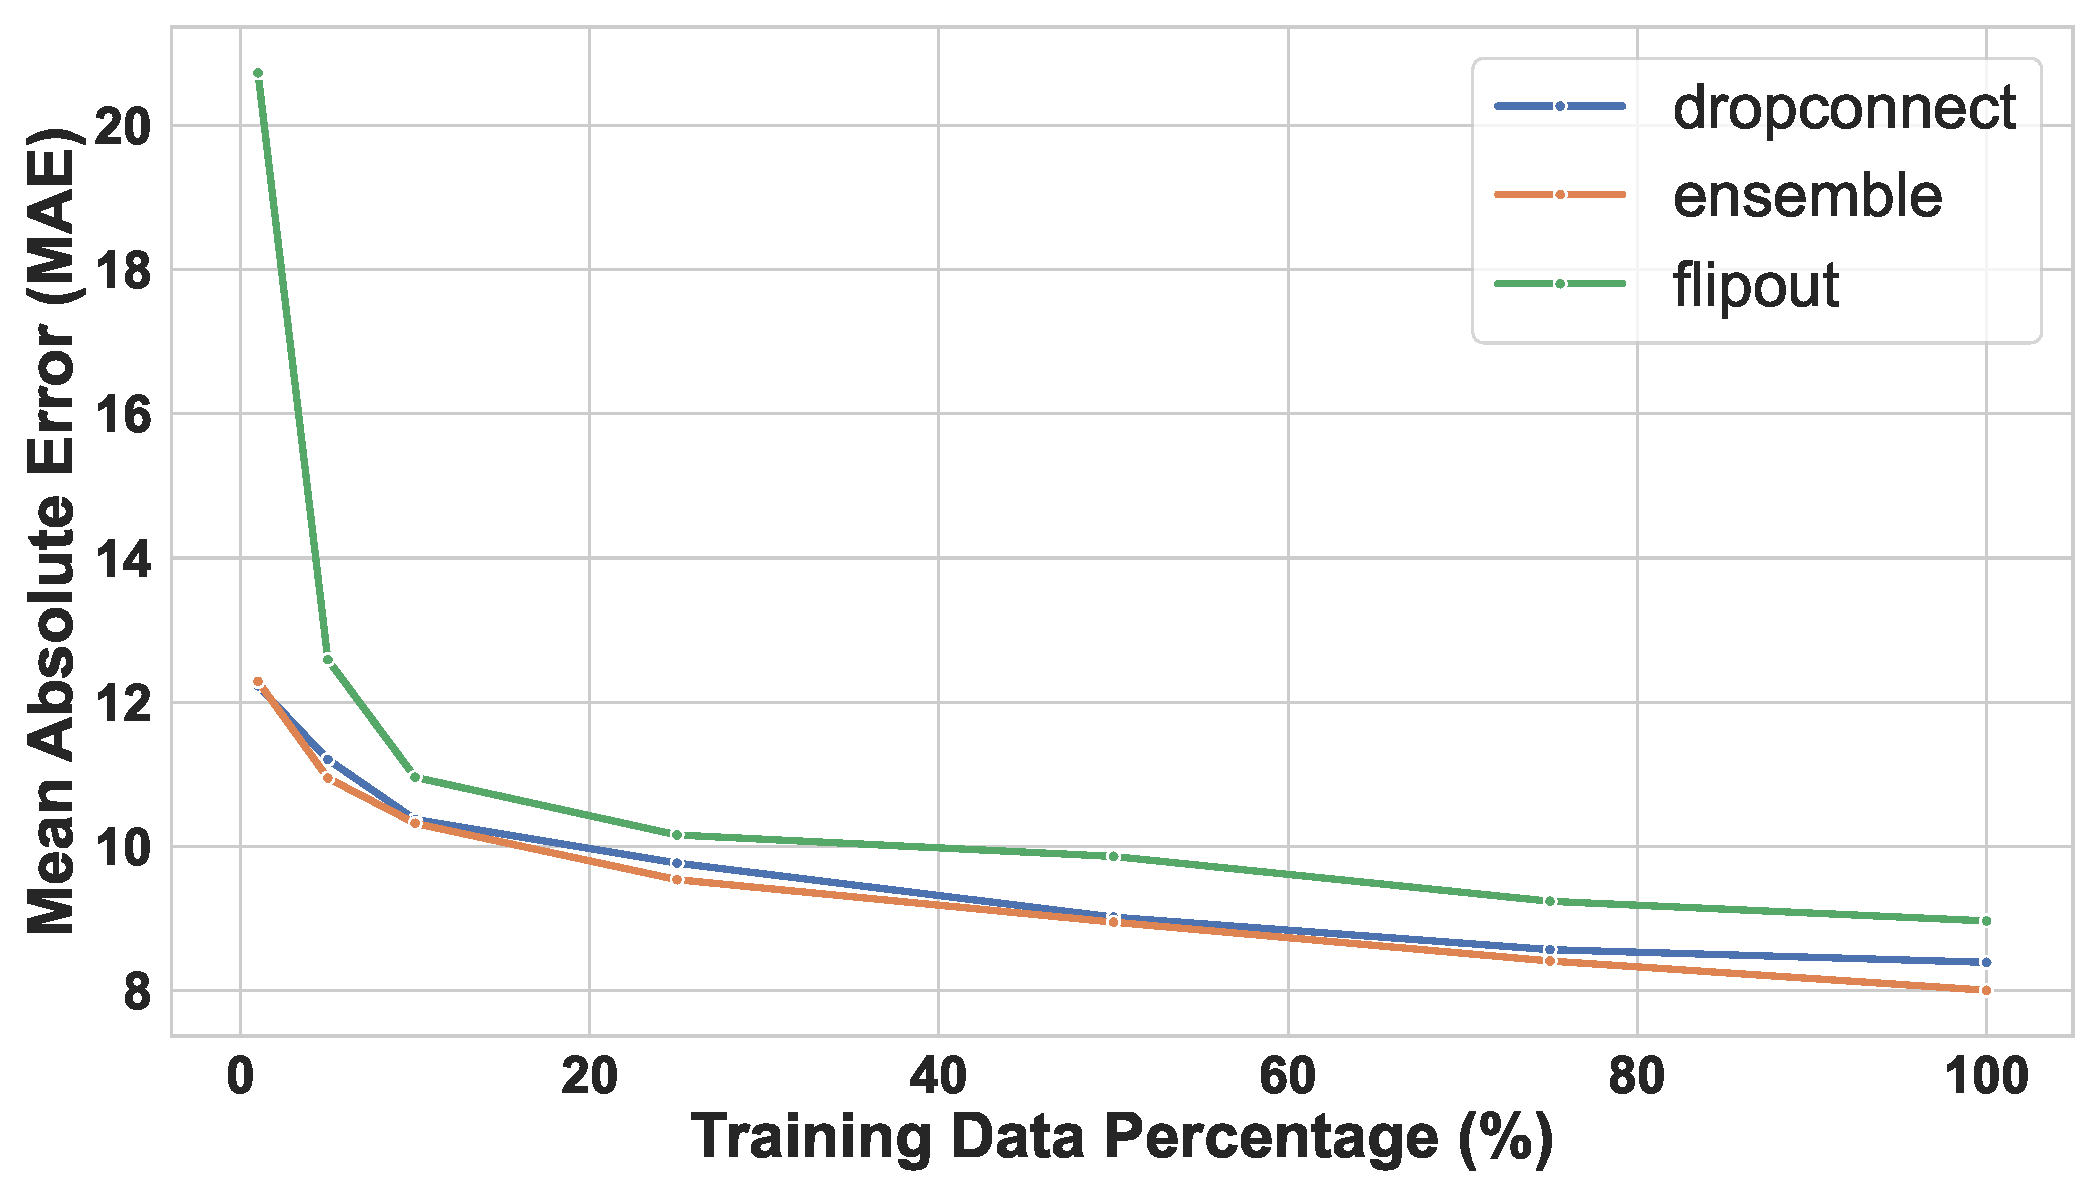
\includegraphics[width=\linewidth]{fig_mae.pdf}
\caption{Mean Absolute Error.}
\end{subfigure}
\hfill
\begin{subfigure}[t]{0.32\linewidth}
\centering
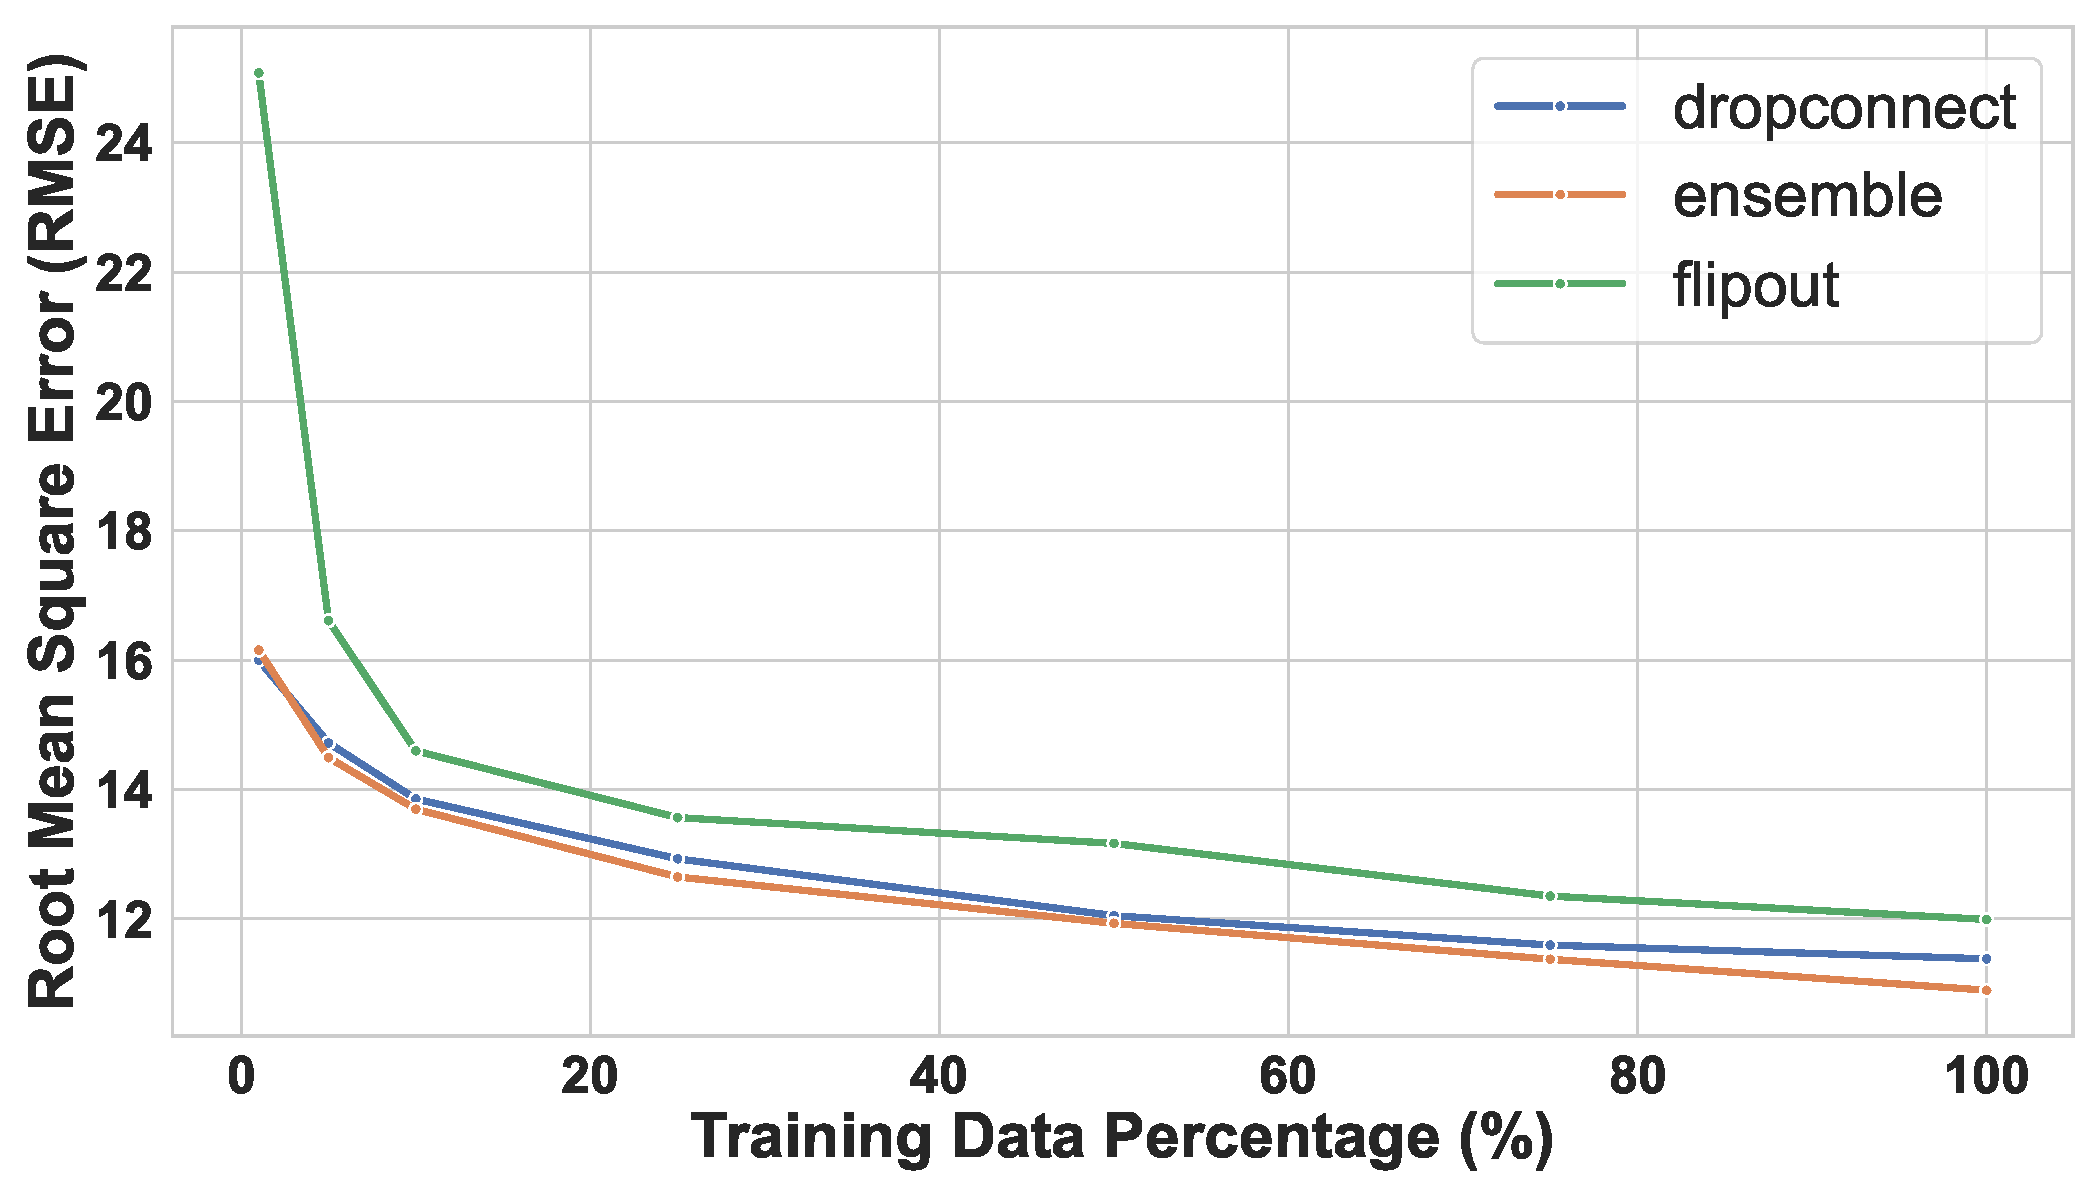
\includegraphics[width=\linewidth]{fig_rmse.pdf}
\caption{Root Mean Squared Error.}
\end{subfigure}
\hfill
\begin{subfigure}[t]{0.32\linewidth}
\centering
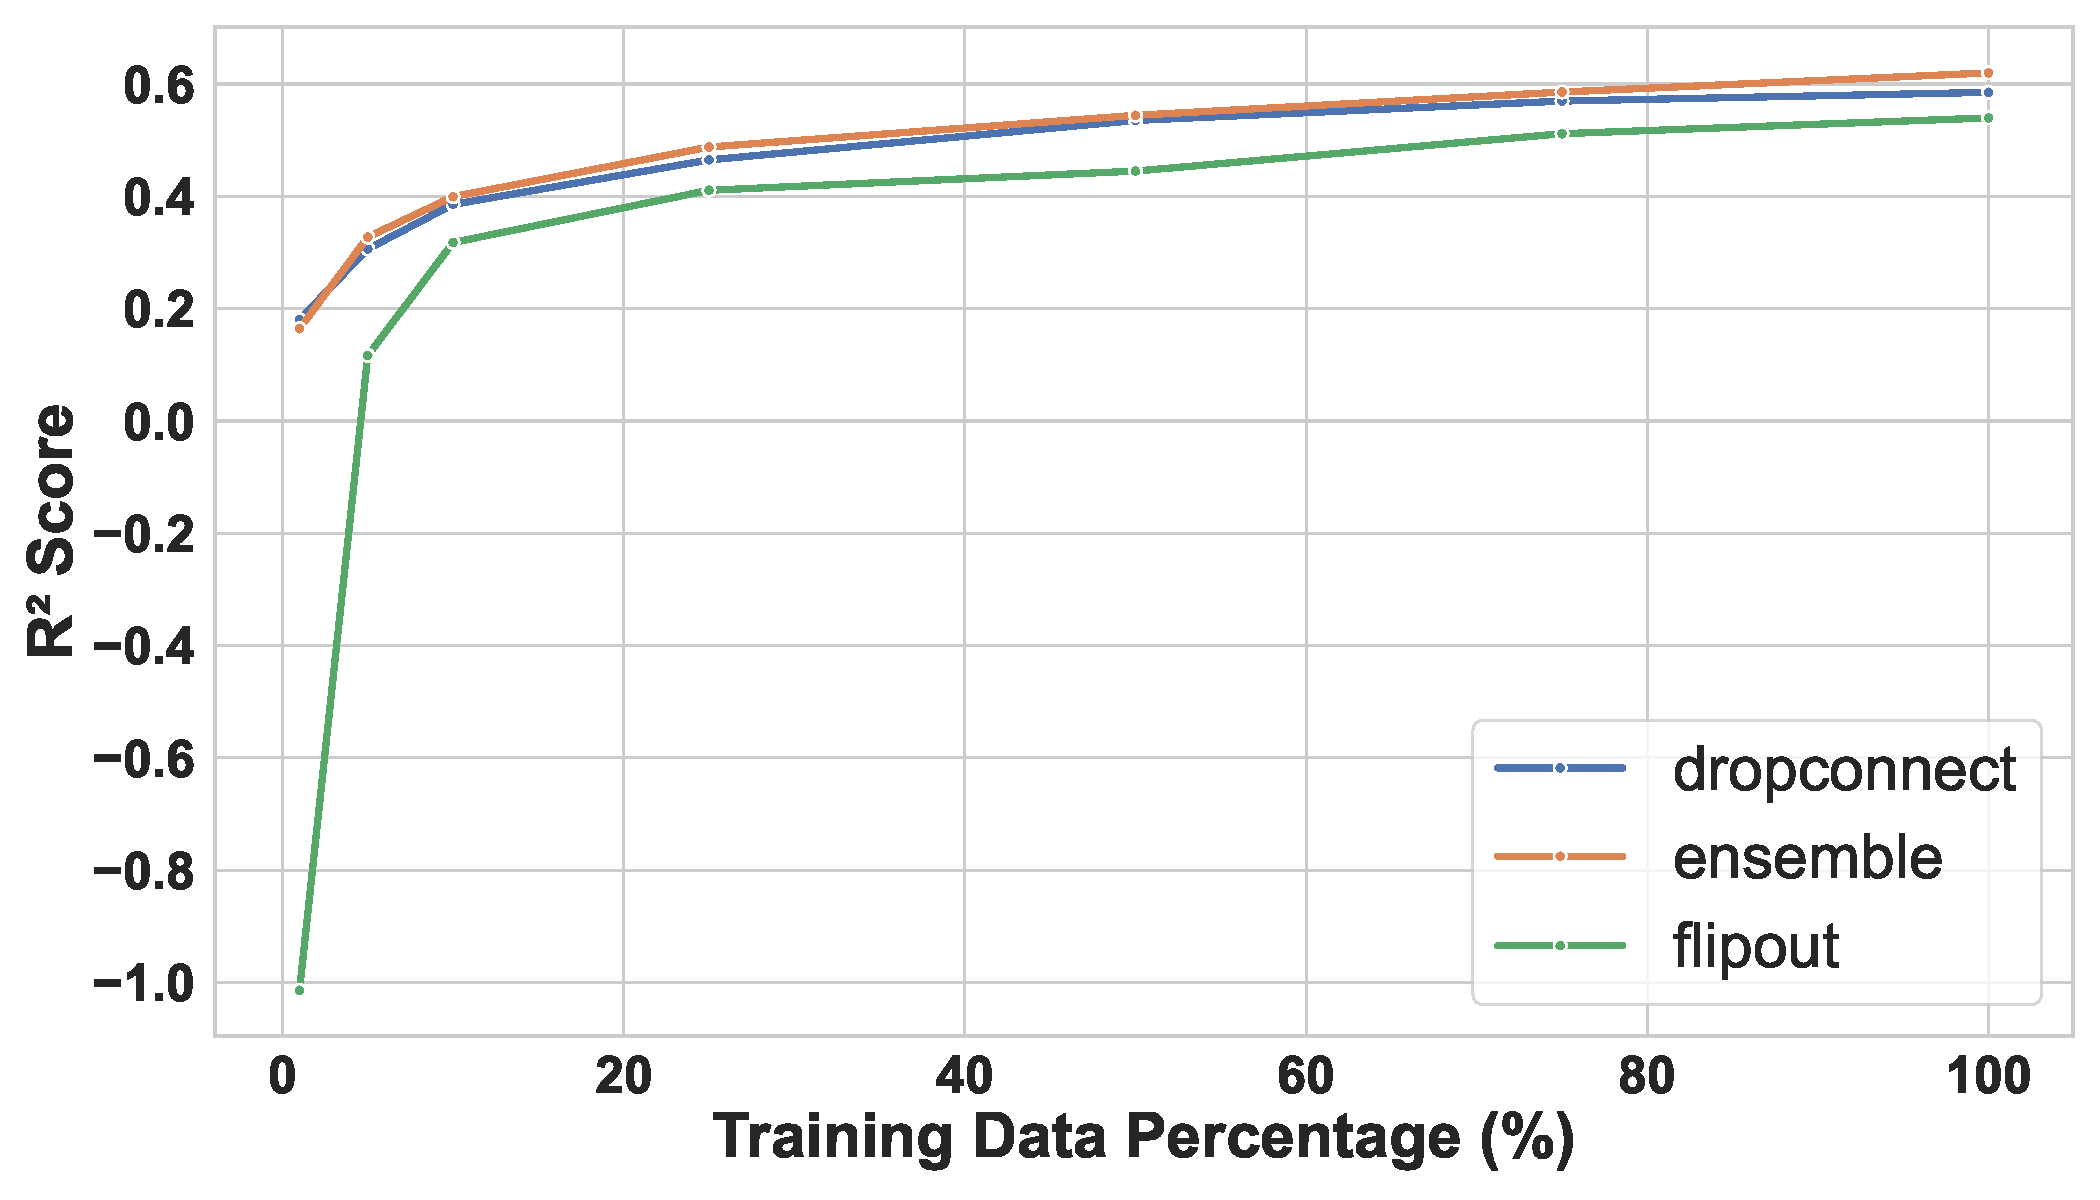
\includegraphics[width=\linewidth]{fig_r2.pdf}
\caption{$R^2$ score.}
\end{subfigure}
\caption{Comparison of metrics across different training set sizes.}
\label{fig:metrics}
\end{figure}

\subsection{Anomalies and Observed Variability}

Despite the overall agreement with theoretical expectations, several notable anomalies and inconsistencies emerged. Most significantly, the Flipout method exhibited non-monotonic behavior in its epistemic uncertainty values. From 10\% to 25\% dataset size, instead of decreasing, epistemic uncertainty rose slightly from 8.72 to 8.99 years, before beginning to decline again. This suggests that Flipout may be more sensitive to factors such as random seed initialization, optimization stability, or model overfitting in intermediate data regimes.

Another anomaly observed in the DropConnect model is that epistemic uncertainty remained relatively high between the 5\% and 10\% data levels. Specifically, the uncertainty decreased only marginally from 12.89 years to 12.02 years, despite the amount of training data doubling. This limited improvement suggests that the model may not have yet reached a sufficiently complex level to benefit from the additional data fully. A more notable reduction in uncertainty becomes apparent only from the 25\% data level onward, indicating that a certain threshold must be crossed before the model can effectively leverage increased data volumes.

Such fluctuations are important to acknowledge, as they reflect the nonlinear and sometimes unstable nature of training Bayesian approximations in neural networks. The presence of these irregularities suggests that further work is needed to improve stability and calibration, especially in low-data regimes.

\subsection{Cross-Dataset Evaluation on UTKFace}
\label{sec:utkface}

\textcolor{red}{\textbf{[TODO -- to be filled once UTKFace runs land.]} This subsection will report the generalisation behaviour of the three uncertainty methods on UTKFace~\cite{zhang2017utkface}, an in-the-wild chronological-age dataset. We assess (i) MAE and RMSE under distribution shift, (ii) calibration of the predicted uncertainty against empirical error, and (iii) representative qualitative cases. The full discussion will be written in the style of the preceding subsections.}

\section{Discussion}
\label{sec:discussion}

This paper investigated whether predictive uncertainty in a regression task can be effectively disentangled into aleatoric and epistemic components. While uncertainty quantification has been widely explored in classification, its interpretability in regression remains comparatively underexamined. The results presented here indicate that regression provides a more favorable setting for uncertainty disentanglement, offering clearer behavioral separation between uncertainty types and more interpretable predictive confidence.

Beyond theoretical relevance, effective uncertainty disentanglement has practical implications. Models that provide calibrated and interpretable uncertainty estimates can significantly enhance trust in real-world deployments. Distinguishing between aleatoric and epistemic uncertainty enables informed decision-making: high aleatoric uncertainty suggests inherently ambiguous inputs, whereas elevated epistemic uncertainty may indicate insufficient data coverage, motivating data collection or model retraining.

\paragraph{Interpretation of Results.}
The empirical trends observed are consistent with theoretical definitions of uncertainty. Aleatoric uncertainty remained largely invariant across different training set sizes, confirming its data-inherent nature, as previously reported by~\cite{kendall2017uncertainties}. Across models and dataset sizes, aleatoric variance stabilized at approximately 18 years squared, corresponding to a standard deviation of 4.2 years, which is plausible given the subjective difficulty of estimating perceived age.

Epistemic uncertainty, in contrast, exhibited the expected inverse relationship with training data size. DropConnect demonstrated a pronounced reduction, decreasing from approximately 12.9 years at 5\% of the data to 6.0 years when trained on the full dataset, reflecting increased model confidence with broader data exposure. Deep Ensembles showed consistently low epistemic uncertainty and reduced sensitivity to data size, likely due to robustness induced by model diversity. Flipout displayed less stable behavior, with non-monotonic fluctuations, particularly at intermediate dataset sizes, suggesting potential instability in its variational inference approximations.

\paragraph{Relation to Existing Literature.}
These findings contrast with prior classification-based studies~\cite{dejong2025measuring}, where strong correlations between aleatoric and epistemic uncertainty hindered successful disentanglement. In the regression setting examined here, the two uncertainty types were substantially more separable, both conceptually and empirically, suggesting that regression tasks may be better suited for uncertainty disentanglement using current approximate Bayesian methods.

The consistently low epistemic uncertainty observed in Deep Ensembles, even under limited data conditions, aligns with previous work by~\cite{lakshminarayanan2017simple}, reinforcing the view that ensembles act as strong non-Bayesian uncertainty approximators. However, this same robustness may mask sensitivity to data scarcity, potentially leading to underestimation of epistemic uncertainty in low-data regimes.

\paragraph{Scalability with More Data.}
A common issue with any machine learning model is the training data and the question of whether more data will improve the model's predictions. Results in Fig.~\ref{fig:metrics}(a) and~\ref{fig:metrics}(b) evaluate standard regression metrics across dataset size, and from these results we can interpolate that the model can continue improving with more data, as the MAE/RMSE slope is negative and does not flatten to indicate possible diminishing gains.

\paragraph{Limitations.}
A key limitation of this study is the reliance on very small training subsets. Models trained on 1\% of the data (approximately 40 samples) exhibited clear underfitting, resulting in unreliable predictions and uncertainty estimates; consequently, these results were excluded from the final analysis. Even at larger subset sizes (5\% and 10\%), Flipout showed irregular and non-monotonic epistemic uncertainty trends, including temporary increases despite additional training data.

The original training relied exclusively on the APPA-REAL dataset, which limits external validity. Although the dataset provides high-quality annotations with low standard error and is well-suited for apparent age estimation, its age distribution is skewed toward individuals aged 20--40, with under-representation of children and elderly adults. This imbalance may impair model generalization and affect uncertainty estimates in sparsely represented age ranges. Our cross-dataset evaluation on UTKFace (Sec.~\ref{sec:utkface}) partially addresses this concern by probing performance and calibration under distribution shift.

Another limitation concerns architectural homogeneity. All experiments employed DenseNet-121 as the backbone architecture due to its efficiency and strong performance. However, uncertainty behavior may depend on architectural properties such as depth, feature reuse, or inductive biases. It therefore remains unclear whether similar disentanglement patterns would emerge with alternative architectures, such as ResNet~\cite{he2016deep} or Vision Transformers~\cite{dosovitskiy2021image}.

Finally, the evaluation lacks a formal quantitative metric for assessing uncertainty disentanglement. The analysis primarily relies on visual inspection and relative comparisons across methods and dataset sizes. Incorporating established disentanglement metrics, such as the disentanglement error proposed by~\cite{dejong2025measuring}, would enable a more rigorous and reproducible evaluation.

\paragraph{Future Work.}
Future research should address these limitations while extending the scope of uncertainty-aware regression modeling. One promising direction is the development of hybrid uncertainty estimation approaches that combine Bayesian and non-Bayesian methods, potentially reducing variance in epistemic estimates while preserving robustness. Ensemble-based Bayesian approximations may offer a balanced trade-off between calibration and stability.

Another important avenue is the personalization of uncertainty estimates. Apparent age perception is inherently subjective and influenced by individual and cultural factors. Future models could adapt uncertainty predictions based on annotator characteristics or contextual information, enhancing interpretability and relevance.

By pursuing these directions, future studies can build upon the findings of our work to improve the reliability, efficiency, and applicability of uncertainty-aware models in age estimation and related regression tasks.

\section{Conclusions}
\label{sec:conclusion}

This work set out to explore whether aleatoric and epistemic uncertainties can be effectively disentangled in a regression setting, specifically within the task of facial apparent age estimation. Building upon prior work that demonstrated limitations in classification contexts, our study focused on regression, where the subjective nature of apparent age offers both a challenge and an opportunity for more interpretable uncertainty modeling.

Our results demonstrate that uncertainty disentanglement is not only feasible in regression but also more stable and interpretable compared to classification. Aleatoric uncertainty remained consistent across all model types and dataset sizes, confirming its origin in data-inherent variability. In contrast, epistemic uncertainty exhibited a clear inverse relationship with training dataset size, decreasing as more data became available. Thus, it validates its dependence on model knowledge and data exposure.

Among the methods evaluated, Deep Ensembles provided the best overall predictive performance and maintained low uncertainty levels, although they appeared less sensitive to changes in training size. DropConnect, although slightly less accurate, showed the most responsive and interpretable epistemic trends, making it a strong candidate for applications that prioritize model confidence estimation. Flipout, on the other hand, showed less stable behavior, particularly at low-data regimes, highlighting limitations in its variational approximation stability.

These findings reinforce the viability of using approximate Bayesian methods to quantify and separate predictive uncertainties in regression tasks. The cross-dataset evaluation on UTKFace further indicates that the learned uncertainty remains informative under distribution shift, an essential property for deployment in real-world settings where input statistics differ from training. As facial age estimation becomes increasingly integrated into high-stakes applications, our study highlights the value of models that can not only predict but also explain their uncertainty.

\subsubsection*{Ethical considerations.}
Facial age estimation can be a controversial topic, as age has historically been used to discriminate persons and age can be private information. The aim of this research is to explore uncertainty estimation in a task that itself is inherently uncertain: humans are not very good at estimating a person's age from just a photo, requiring the concept of apparent age. Machine Learning models can to some degree estimate a person's age from a facial image, but models are not better than humans and should not be used for any kind of automated processing or discriminatory activities.

Uncertainty estimation usually improves the trustworthiness of a model, as the model can now express a confidence interval for the answer instead of a point estimate, and a human user receives information about the model being not sure about its output, and this information can be used to weight the usefulness of a prediction.

This paper only uses data from the APPA-REAL and UTKFace datasets and no human subjects were directly involved in this research.

\bibliographystyle{splncs04}
\bibliography{references}

\end{document}
